\documentclass[11pt,a4paper]{article}
\usepackage[utf8]{inputenc}
\usepackage[T1]{fontenc}
\usepackage{lmodern}
\usepackage{amsmath,amssymb,amsfonts,amsthm}
\usepackage{geometry}
\geometry{margin=1in}
\usepackage{xcolor}
\usepackage{hyperref}
\usepackage{cleveref}
\usepackage{booktabs}
\usepackage{array}
\usepackage{cite}
\usepackage{microtype}
\usepackage{tcolorbox}
\usepackage{slashed}

\hypersetup{
    colorlinks=true,
    linkcolor=blue,
    citecolor=red,
    urlcolor=cyan,
    pdftitle={Lattices, T-Duality, and Double Field Theory on K3 x T2: A Lean 4 Companion Formalization},
    pdfauthor={Xavier Callens and the SocrateAI Scientific Agora Collaboration}
}

\newtheorem{theorem}{Theorem}[section]
\newtheorem{lemma}[theorem]{Lemma}
\newtheorem{definition}[theorem]{Definition}
\newtheorem{proposition}[theorem]{Proposition}
\newtheorem{corollary}[theorem]{Corollary}
\newtheorem{conjecture}[theorem]{Conjecture}

\theoremstyle{remark}
\newtheorem{remark}[theorem]{Remark}

% ---------------------------------------------------------------------------
% Epistemic tier badges, following the convention of paper 7
% (papers/publication/paper7_dual_scale_theory_master_demonstration.tex)
% and docs/PAPER_REVISION_BRIEF_2026_09_17.md §0.
% ---------------------------------------------------------------------------
\newcommand{\tierA}{\colorbox{green!15}{\textsf{\scriptsize Tier A --- Lean kernel}}}
\newcommand{\tierL}{\colorbox{blue!10}{\textsf{\scriptsize Tier L --- literature}}}
\newcommand{\tierC}{\colorbox{orange!15}{\textsf{\scriptsize Tier C --- conjecture}}}
\newcommand{\tierS}{\colorbox{gray!15}{\textsf{\scriptsize symbolic check (sympy), not Tier A}}}

\newtcolorbox{scopebox}{%
  colback=gray!5, colframe=gray!45, boxrule=0.4pt, arc=1pt,
  left=6pt, right=6pt, top=3pt, bottom=3pt,
  fonttitle=\bfseries\small, title={Scope of Lean 4 verification}
}

\title{\Huge \textbf{Lattices, T-Duality, and Double Field Theory}\\[0.3em]
\LARGE \textbf{on $K3\times T^2$:}\\[0.2em]
A Lean~4 Companion Formalization}

\author{\textbf{Xavier Callens}$^{1}$ \and \textbf{SocrateAI Scientific Agora Collaboration}$^{1}$ \\[0.5em]
$^{1}$\textit{SocrateAI Research Laboratory for Mathematical Physics \& Formal Verification}}

\date{Revision 2 --- September 18, 2026}

\usepackage{graphicx}
\graphicspath{{../book/generated/figures/}}
% [layout] allow long Lean identifiers to break after underscores (added 2026-09-17)
\makeatletter\let\LMoldunderscore\_\renewcommand{\_}{\LMoldunderscore\allowbreak}\makeatother
\setlength{\emergencystretch}{3em}
% [/layout]
\begin{document}

\maketitle

\begin{abstract}
Closed-string compactification on $K3\times T^2$ carries, besides its continuous geometric
moduli, a discrete duality structure: T-duality identifies backgrounds related by
$R\leftrightarrow \alpha'/R$ and, more generally, by the arithmetic group $O(d,d;\mathbb{Z})$
acting on the lattice of momentum and winding charges. We report a Lean~4 library,
\texttt{DualScaleStream2} (19 modules, built on Mathlib, toolchain \texttt{v4.33.1}), that
kernel-checks the algebraic skeleton underlying this structure: positive-definiteness and
unimodularity of the $E_8$ and hyperbolic lattices that build $H^2(K3,\mathbb{Z})$; the
signature arithmetic of the K3, Mukai, and $K3\times T^2$ charge lattices; the $O(d,d;\mathbb{Z})$
generators of Giveon--Porrati--Rabinovici and their charge-norm and spectrum invariance; the
Hull--Zwiebach generalized metric of Double Field Theory and its $B$-field shifts and section
condition; a $d$-dimensional trace-bound generalization, $\operatorname{tr}G+\operatorname{tr}G^{-1}\ge 2d$,
of the one-dimensional statement behind this research programme's ``dual-scale'' proposal; flux
integrality and D-brane tadpole counting on $K3\times T^2$ and $K3\times K3$; and the arithmetic
of the Eguchi--Ooguri--Tachikawa Mathieu-moonshine coefficients. All 100 theorems are accepted by
the Lean~4 kernel with zero \texttt{sorry} and an axiom footprint limited to Lean's three
standard axioms (\texttt{propext}, \texttt{Classical.choice}, \texttt{Quot.sound}). We state
throughout, and repeat in a dedicated section, what this formalization does and does not
establish: every statement is about finite-dimensional matrices over $\mathbb{Z}$ or $\mathbb{R}$;
the identification of these matrices with string-theory charge lattices, dualities, and
background fields is quoted from the literature (Tier~L) or is this project's own reading
(Tier~C), never re-derived as physics. We also report, as part of the methods, the tiered
multi-agent pipeline that produced these proofs and its measured failure modes: a cheap local
prover closes concrete goals and nothing symbolic, and two agent self-reports of successful
compilation were false and caught only because every claim was independently recompiled.
\end{abstract}

\newpage
\tableofcontents
\newpage

\section*{Revision note (Revision 2, 2026-09-18)}
An external review of the first version (recorded verbatim, with a point-by-point response, in
\texttt{docs/reviews/} of the repository) was favourable but read several results as stronger than
they were. This revision responds as follows.
\begin{enumerate}
  \item The review stated that the trace bound is ``minimized exactly at the self-dual point.'' The
    first version proved attainment at $G=\mathbf 1_d$ only, and said so. \textbf{That gap is now
    closed}: the new theorem \texttt{dualScale\_eq\_iff} proves
    $\mathcal{D}(G)=2d\iff G=\mathbf 1_d$ for positive-definite $G$ (\Cref{sec:trace-bound}). The
    library has 100 theorems, not 99.
  \item The review called Tier~A ``absolute mathematical certainty'' and the library ``bulletproof,
    bug-free.'' We do not accept either description; \Cref{sec:tiers} now states the trust base of
    a Tier~A claim and adds these phrases to the list this paper does not use.
  \item The review said false agent reports were ``caught 100\% of the time.'' That rate cannot be
    known, and \Cref{sec:methods} now says why and what is guaranteed instead. It also described the
    orchestrator as human; it was a model, working under the author's direction, as
    \Cref{sec:methods} already stated.
\end{enumerate}
Three further readings in the review are corrected in the response document rather than here,
because this paper already stated them correctly: the hyperbolic plane $U$ is indefinite, not
definite (\Cref{sec:lattices}); the lattice signatures are bookkeeping on Tier~L inputs, not computed
from Gram matrices; and the moonshine module checks an arithmetic coincidence, it does not validate
the moonshine observation.

%%%%%%%%%%%%%%%%%%%%%%%%%%%%%%%%%%%%%%%%%%%%%%%%%%%%%%%%%%%%%%%%%%%%%%%%%%%%%%%
\section{Introduction}
\label{sec:intro}
%%%%%%%%%%%%%%%%%%%%%%%%%%%%%%%%%%%%%%%%%%%%%%%%%%%%%%%%%%%%%%%%%%%%%%%%%%%%%%%

\subsection{The physical question}
A closed string propagating on a circle of radius $R$ has momentum modes $n\in\mathbb{Z}$ and
winding modes $w\in\mathbb{Z}$, with mass spectrum invariant under the simultaneous exchange
$R\leftrightarrow \alpha'/R$, $n\leftrightarrow w$: the Buscher T-duality
\cite{Buscher1987,Buscher1988}. Two geometrically distinct backgrounds --- a large circle and a
small one --- describe the same conformal field theory. On a $d$-torus this discrete symmetry
grows into the arithmetic group $O(d,d;\mathbb{Z})$ acting on the $2d$-dimensional lattice of
momenta and windings, preserving the split-signature pairing that couples the two
\cite{Narain1986,GiveonPorratiRabinovici1994}. Compactifying further on a $K3$ surface adds a
second, richer duality structure: the moduli space of $(0,4)$ or $(4,4)$ superconformal field
theories on $K3$ is (conjecturally, and in restricted regimes provably) a double coset of the
orthogonal group of an even lattice of signature $(3,19)$, and type~IIA/IIB and heterotic strings
on $K3\times T^2$ or $K3\times T^3$ are related by a web of string-string and string-M-theory
dualities in which $T$-duality, $S$-duality, and geometric monodromies of $K3$ all appear as
elements of a single arithmetic group \cite{Aspinwall1996}. Hull and Zwiebach's Double Field
Theory (DFT) makes the $O(d,d)$ structure manifest at the level of the low-energy effective
action, by doubling the torus coordinates and packaging the metric $G$ and Kalb--Ramond field
$B$ into a single \emph{generalized metric} $\mathcal{H}(G,B)$ valued in the coset
$O(d,d)/(O(d)\times O(d))$ \cite{HullZwiebach2009}.

This research programme's own recurring theme --- explored in Stream~1's Lean corpus and its
companion paper 7 \cite{Callens2026Paper7} --- is that the self-dual point of this duality,
$R=\sqrt{\alpha'}$, marks a minimum of an effective length scale $R_{\mathrm{eff}}=R+\alpha'/R$,
suggestively read as a stringy obstruction to reaching arbitrarily short distances. The present
paper reports a second, independent Lean~4 library, \texttt{DualScaleStream2}, that (a) builds the
lattice-theoretic scaffolding of $K3\times T^2$ compactification from first principles ($E_8$,
the hyperbolic plane $U$, their direct sums), (b) formalizes the $O(d,d;\mathbb{Z})$ duality group
and the Hull--Zwiebach generalized metric for \emph{every} $d$, not just $d=1$, and (c) proves a
$d$-dimensional generalization of the dual-scale bound, $\operatorname{tr}G+\operatorname{tr}G^{-1}\ge 2d$,
that specializes exactly to Stream~1's circle statement. It also revisits, with a corrected and
more carefully sourced arithmetic, the Mathieu-moonshine decomposition of the $K3$ elliptic genus
and the flux/tadpole counting of $K3\times T^2$ orientifolds.

\subsection{What a machine-checked formalization adds, and what it does not}
A Lean~4 kernel proof adds a very specific and narrow guarantee: that a stated fact about
matrices, vectors, and rational or real arithmetic follows from the axioms of Lean's core logic
plus (in this library) Mathlib's development of linear algebra, by an explicit, machine-verified
derivation with no unproven step (\texttt{sorry}) and no undisclosed extra axiom. It does not, by
itself, establish that the matrices in question \emph{are} the charge lattices, dualities, or
background fields of any string theory --- that identification is supplied by the physics
literature we cite, and is stated here as such throughout. Nor does formalizing an algebraic
identity establish the deeper facts that make it interesting: that $O(d,d;\mathbb{Z})$ is
generated by the elements we exhibit (Giveon--Porrati--Rabinovici prove this; we do not
re-derive it), that Sylvester's law of inertia correctly reads off a lattice's signature from a
diagonal congruence (we use it, we do not reprove it), or that the $K3$ elliptic genus really
carries an $M_{24}$ action (Eguchi--Ooguri--Tachikawa's observation, proved by Gannon
\cite{Gannon2016}). We adopt the same three-tier epistemic convention as paper~7, restated below
for a self-contained reading, and follow it strictly: every claim in this paper is labelled, and
a claim never rests, even transitively, on a lower tier without that dependency being stated.

\subsection{Epistemic tiers}
\label{sec:tiers}
\begin{itemize}
  \item \tierA\ --- \textbf{Lean kernel}: the exact stated declaration is accepted by the Lean~4
    kernel (\texttt{v4.33.1}, Mathlib \texttt{v4.33.1}), with zero \texttt{sorry}, and
    \texttt{\#print axioms} shows only \texttt{propext}, \texttt{Classical.choice}, and
    \texttt{Quot.sound} (\Cref{app:repro}). Tier~A is a claim about the cited Lean declaration,
    not automatically about the informal sentence next to it: where a theorem proves only one
    direction of an ``iff'', or a bound over a strict subset of cases, this paper says so.
  \item \tierL\ --- \textbf{literature}: quoted from a cited paper, by section/equation and by
    file/line into the \texttt{papers/foundations/*.txt} extraction used to write this
    corpus, not independently re-derived here.
  \item \tierC\ --- \textbf{conjecture}: this project's own interpretation, physical reading, or
    unproven proposal.
\end{itemize}
A fourth marker, \tierS, flags a small number of matrix-convention checks (sign and transpose
placements) that were verified with \texttt{sympy} \emph{before} the Lean statement was written,
as a sanity check on the formalization choice, and are explicitly \emph{not} Tier~A: a symbolic
computer-algebra check is not a kernel proof, and this paper never cites one as if it were.

\textbf{What a Tier~A claim rests on.} Tier~A is not ``absolute certainty.'' It is certainty
\emph{relative to} a stated trust base: the soundness of Lean's type theory and the correctness of
its kernel implementation at this version, the three standard axioms, the Mathlib definitions the
statement is written in, and --- the part no kernel can check --- that the formal statement says what
the prose next to it says. The last item is where every error this project has actually found
occurred (a mistyped $M_{24}$ table, a \texttt{Nat}-truncated ``unique'' minimum, a source equation
transcribed with the wrong exponent in a later library), and it is why statements are reviewed
against their sources and then hash-locked (\Cref{app:repro}).

\textbf{Forbidden phrasings.} Following \texttt{docs/PAPER\_REVISION\_BRIEF\_2026\_09\_17.md} \S0,
this paper does not use the phrases ``zero axioms,'' ``100\% mathematical rigor,'' ``certifies
stability,'' ``formalizes string theory,'' ``first fully certified,'' ``all of physics,''
``absolute certainty,'' ``bulletproof,'' or ``bug-free.'' The
correct form used throughout is: proved in Lean~4 with no axioms beyond Lean's three standard
axioms, with the string-theoretic reading of each proved statement stated separately and tiered.

\subsection{Relation to the Stream~1 corpus: why this library uses Mathlib}
Paper~7's corpus (\texttt{StringTheoryFoundation}, \texttt{DoubleFieldTheory},
\texttt{DualScaleM24Formalization}, \texttt{DualScaleValidation}, \texttt{Lean5Corpus},
\texttt{StringTheoryFormalization}) deliberately has \emph{no} Mathlib dependency, so every
statement there is over \texttt{Nat}, \texttt{Int}, or an ad hoc rational-pair structure; its
circle-bound theorem, \texttt{UseCase1.self\_dual\_is\_global\_minimum}, is consequently only an
$\mathbb{N}$-instance ($R\ge 1\Rightarrow R^2+1\ge 2$), not a real bound. \texttt{DualScaleStream2}
is a new, separate \texttt{lean\_lib} that \emph{imports} Stream~1 (never the reverse, so
Stream~1's build cannot be broken by Stream~2 work) and additionally imports Mathlib, specifically
to reach real-number linear algebra: positive-definite matrices, matrix inverses, traces, and
transposes. This is the direct, disclosed reason \Cref{sec:trace-bound}'s bound is a genuine
statement over $\mathbb{R}$ for every positive-definite $d\times d$ matrix $G$
(\texttt{DualScale.dualScale\_ge}, \texttt{DualScale.circle\_effective\_scale\_ge\_two}), where
paper~7's analogous statement remained an integer instance pending exactly this step. We regard
this as the two corpora being complementary rather than in tension: Stream~1 demonstrates what
can be proved with \emph{no} external dependency; Stream~2 demonstrates what the same
programme's central claims look like once Mathlib is available.

The remainder of this paper proceeds one formalized layer at a time (lattices,
\Cref{sec:lattices}; T-duality, \Cref{sec:tduality}; Double Field Theory,
\Cref{sec:dft}; the dual-scale bound, \Cref{sec:trace-bound}; flux and tadpole,
\Cref{sec:flux}; Mathieu moonshine, \Cref{sec:moonshine}), each with the ordinary-notation
mathematics, its physical motivation, and a table mapping every cited Lean declaration to its
tier. \Cref{sec:scope} then collects, in one place, an explicit statement of what is and is not
proved. \Cref{sec:methods} describes the tiered multi-agent pipeline that produced the corpus and
its measured results, including its failures. \Cref{app:repro} gives exact reproduction
commands and numbers.

Throughout, charge vectors are ordered momentum $\oplus$ winding, and the $O(d,d)$-invariant form
is $\eta=\begin{pmatrix}0 & \mathbf{1}_d\\ \mathbf{1}_d & 0\end{pmatrix}$.

%%%%%%%%%%%%%%%%%%%%%%%%%%%%%%%%%%%%%%%%%%%%%%%%%%%%%%%%%%%%%%%%%%%%%%%%%%%%%%%
\section{Lattices for $K3\times T^2$}
\label{sec:lattices}
%%%%%%%%%%%%%%%%%%%%%%%%%%%%%%%%%%%%%%%%%%%%%%%%%%%%%%%%%%%%%%%%%%%%%%%%%%%%%%%

\subsection{Why lattices}
The charge lattices of string compactification --- $H^2$ of a $K3$ surface, the Narain lattice of
a torus, the lattice of D-brane charges --- are even, unimodular (self-dual) lattices of
indefinite signature, and their isometry groups are exactly the duality groups of the physical
theory. Two building blocks recur throughout the subject: the negative-definite $E_8$ root
lattice $E_8(-1)$, and the rank-2 hyperbolic plane $U$ with Gram matrix
$\begin{pmatrix}0&1\\1&0\end{pmatrix}$. Huybrechts records the resulting decomposition of the K3
lattice,
\begin{equation}
  H^2(K3,\mathbb{Z}) \;\cong\; E_8(-1)^{\oplus 2}\oplus U^{\oplus 3},
\end{equation}
an even, unimodular lattice of rank 22 and signature $(3,19)$ (Huybrechts, \emph{Lectures on K3
Surfaces}, Ch.~1, eq.~(3.4), \texttt{huybrechts\_K3Global.txt} l.~603) \cite{Huybrechts}. Its
orthogonal group, and in particular the subgroup fixing a choice of polarization, is the discrete
part of the $K3$ moduli space and of the string dualities acting on it
(Aspinwall, \emph{K3 Surfaces and String Duality}, hep-th/9611137, ll.~705--766, 1737--1748)
\cite{Aspinwall1996}.

\subsection{$E_8$: unimodularity, positive-definiteness, and the exact determinant}
\label{sec:e8}
$E_8$ is the rank-8 integral lattice with Cartan/Gram matrix
\begin{equation}
  \mathrm{cartanE8} =
  \begin{pmatrix}
   2&-1&0&0&0&0&0&0\\
   -1&2&-1&0&0&0&0&0\\
   0&-1&2&-1&0&0&0&0\\
   0&0&-1&2&-1&0&0&0\\
   0&0&0&-1&2&-1&0&-1\\
   0&0&0&0&-1&2&-1&0\\
   0&0&0&0&0&-1&2&0\\
   0&0&0&0&-1&0&0&2
  \end{pmatrix}.
\end{equation}
Rather than asserting $\det=\pm 1$, \texttt{DualScaleStream2} certifies unimodularity the way
\texttt{Lattice.Basic.isUnimodular\_of\_mul\_eq\_one} makes canonical for the whole corpus: an
explicit integer matrix \texttt{cartanE8Inv} is exhibited, and the kernel checks
\texttt{cartanE8Inv * cartanE8 = 1} entry by entry (\texttt{cartanE8Inv\_mul}); an integer left
inverse forces $\det=\pm1$ by \texttt{isUnimodular\_of\_mul\_eq\_one}. This certificate-based
style means a wrong inverse would simply fail to typecheck rather than silently asserting a false
determinant. The matrix is symmetric (\texttt{cartanE8\_symm}) with even diagonal
(\texttt{cartanE8\_evenDiag}), so by \texttt{even\_quadratic\_form\_of\_even\_diag} every integer
vector has even norm --- $E_8$ is an even lattice. The sign-reversed lattice $E_8(-1)$, the
summand that actually appears in $H^2(K3,\mathbb{Z})$, inherits all three properties
(\texttt{e8Neg\_symm}, \texttt{e8Neg\_evenDiag}, \texttt{e8Neg\_unimodular}).

Unimodularity alone does not distinguish $E_8$ from an indefinite even unimodular lattice of the
same rank; the physically relevant fact is that $E_8$ is \emph{positive definite} (so $E_8(-1)$ is
negative definite, matching its role in the signature-$(3,19)$ decomposition). This is proved by
an exact rational $LDL^\mathsf{T}$ factorization over $\mathbb{R}$,
$D=\operatorname{diag}\!\left(2,\tfrac32,\tfrac43,\tfrac54,\tfrac65,\tfrac76,\tfrac87,\tfrac18\right)$,
with all eight pivots strictly positive and product $1$ (\texttt{e8\_LDL}, \texttt{cartanE8\_det}
$:\ \mathtt{cartanE8.det}=1$ over $\mathbb{Z}$). Positive-definiteness of the real matrix
\texttt{cartanE8R} (the $\mathbb{Z}\to\mathbb{R}$ cast of \texttt{cartanE8}) is then proved
(\texttt{cartanE8\_posDef}) via the sum-of-squares identity
\begin{equation}
  x^{\mathsf T} E_8\, x = 2y_0^2+\tfrac32 y_1^2+\tfrac43 y_2^2+\tfrac54 y_3^2+\tfrac65 y_4^2+\tfrac76 y_5^2+\tfrac87 y_6^2+\tfrac18 y_7^2,
\end{equation}
each $y_k$ an explicit linear form in $x$ from the back-substitution of the factorization, checked
by \texttt{ring} and then completed by an explicit back-substitution argument that a vanishing sum
of these eight squares forces $x=0$.

\subsection{The hyperbolic plane $U$}
$U=\begin{pmatrix}0&1\\1&0\end{pmatrix}$ is even (\texttt{hyperbolicU\_evenDiag}), symmetric
(\texttt{hyperbolicU\_symm}), and its own inverse, hence unimodular
(\texttt{hyperbolicU\_mul\_self}, \texttt{hyperbolicU\_unimodular}). A rational congruence witness
$P^{\mathsf T}UP=\operatorname{diag}(2,-2)$ with $P=\begin{pmatrix}1&1\\1&-1\end{pmatrix}$
(\texttt{hyperbolicU\_congruence}) exhibits one positive and one negative diagonal entry; reading
off the lattice's signature $(1,1)$ from this diagonal congruence is an instance of Sylvester's
law of inertia, which is \tierL, not re-proved here. Separately,
\texttt{hyperbolicU\_eq\_narain\_gram} proves that this $U$ is, on the nose, the Gram matrix
already certified as the Narain lattice $\Gamma^{1,1}$ in Stream~1's
\texttt{StringTheoryFormalization.UseCases.NarainLattice} --- Stream~2 builds on that fact rather
than restating it.

\subsection{Signature bookkeeping: K3, Mukai, and $K3\times T^2$}
% [fig:e8_k3_gram] generated by tools/insert_paper_figures.py from tools/book_figures.py
\begin{figure}[tbp]
\centering
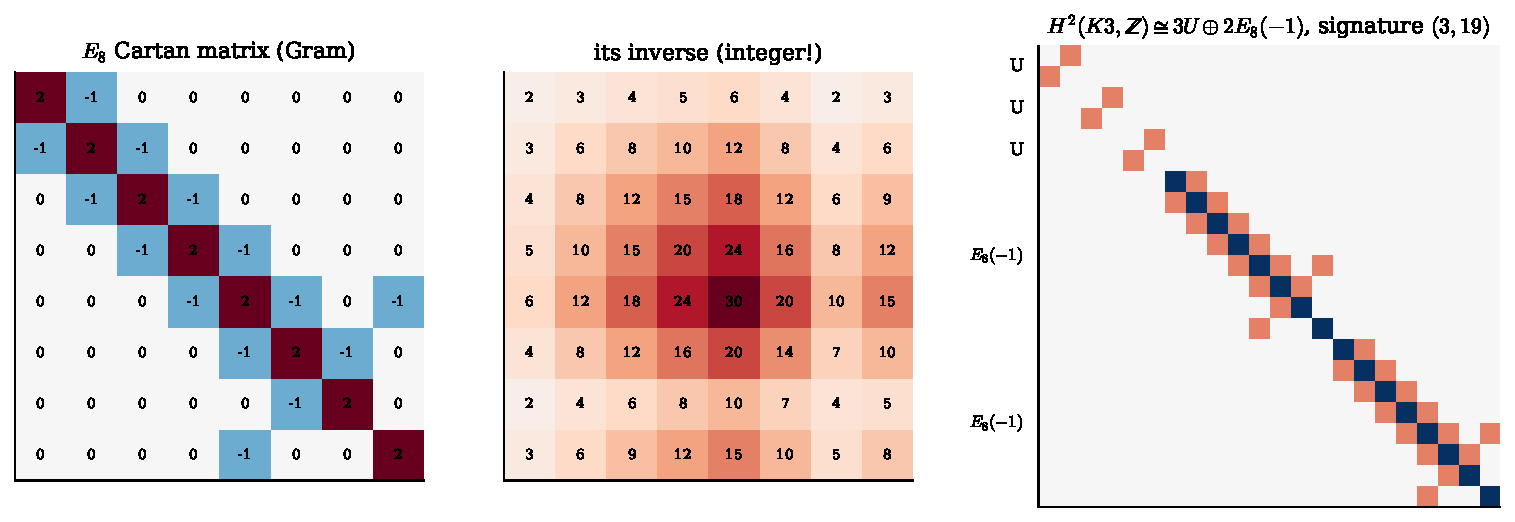
\includegraphics[width=\linewidth]{e8_k3_gram.pdf}
\caption{Left: the Gram matrix of $E_8$ (the Cartan matrix used in Lean) and its inverse, which has integer entries because $\det=1$ (unimodularity). Right: the $22\times22$ Gram matrix of the K3 lattice $3U\oplus2E_8(-1)$ (red $+$, blue $-$); even diagonal, determinant $\pm1$, signature $(3,19)$. \emph{Computed figure; data: Lean \texttt{cartanE8} (E8.lean), \texttt{hyperbolicU} (Hyperbolic.lean); \texttt{cartanE8Inv\_mul}, \texttt{sigK3\_eq}.}}
\label{fig:e8_k3_gram}
\end{figure}
% [/fig:e8_k3_gram]
\texttt{Lattice.K3T2Signature} introduces a small \texttt{Signature} structure (a pair of
naturals, positive/negative multiplicity) and computes, purely arithmetically, the signatures of
\begin{align}
  \mathrm{sigK3} &= E_8(-1)\oplus E_8(-1) \oplus U\oplus U\oplus U, \\
  \mathrm{sigMukai} &= \mathrm{sigK3}\oplus U, \\
  \mathrm{sigT2} &= U\oplus U, \\
  \mathrm{sigK3T2} &= \mathrm{sigMukai}\oplus \mathrm{sigT2},
\end{align}
where the component signatures $U=(1,1)$ and $E_8(-1)=(0,8)$ are Tier~L inputs (established
above only for the individual lattice-theoretic facts unimodular/even/positive-definite, not for
the signature label itself, which uses Sylvester's law). The results,
$\mathrm{sigK3}=(3,19)$, $\mathrm{sigMukai}=(4,20)$, and $\mathrm{sigK3T2}=(6,22)$
(\texttt{sigK3\_eq}, \texttt{sigMukai\_eq}, \texttt{sigK3T2\_eq}, each proved by \texttt{rfl} on
the additive structure), reproduce the Mukai lattice $\Gamma^{4,20}$ and the $K3\times T^2$
charge lattice $\Gamma^{6,22}$ of the physics literature (Aspinwall, ll.~1737--1748), of ranks
22 and 28 respectively (\texttt{rank\_K3}, \texttt{rank\_K3T2}). All three signatures satisfy the
index condition $b_+-b_-\equiv 0\pmod 8$ (\texttt{index\_mod\_eight}) required of an even
unimodular indefinite lattice by the Milnor--Serre classification (not downloaded; cited by
reference only) --- again arithmetic on the already-computed pairs, not a re-derivation of the
classification theorem itself.

A genuine cross-check, not merely a restatement, is \texttt{sigK3\_matches\_hodge}: the
lattice-decomposition signature $(3,19)$ agrees, component by component, with the
\emph{Hodge-theoretic} signature $(2h^{2,0}+1,\,h^{1,1}-1)$ already computed independently in
Stream~1's \texttt{StringTheoryFormalization.UseCases.K3Signature}. As the module's own docstring
states, this is agreement between two independently tabulated Tier~L inputs (the lattice
decomposition and the Hodge diamond), not an independent derivation of either.

\subsection{The Mukai pairing}
On the extended lattice $H^0\oplus H^2\oplus H^4$, Huybrechts's Mukai pairing on a vector
$v=(r,c,s)$ is $\langle v,w\rangle = c\cdot L\cdot c' - rs'-sr'$ (Huybrechts,
\emph{Lectures on K3 Surfaces}, Ch.~9 \S1, Def.~1.4, chapter heading l.~7352, definition
ll.~7475--7482), with Hirzebruch--Riemann--Roch reading $\chi(E,F)=-\langle v(E),v(F)\rangle$.
\texttt{Lattice.Mukai} represents a Mukai vector as a structure \texttt{MukaiVec}
$(r:\mathbb{Z},\,c:\mathrm{Fin}\,n\to\mathbb{Z},\,s:\mathbb{Z})$ and proves the pairing
\texttt{mukaiPair} symmetric for symmetric $L$ (\texttt{mukaiPair\_symm}), with self-pairing
$v^2=c\cdot L\cdot c-2rs$ (\texttt{mukaiPair\_self}), and even whenever $L$ is even
(\texttt{mukaiPair\_even}, reusing \texttt{even\_quadratic\_form\_of\_even\_diag}). The
$H^0\oplus H^4$ summand $U(-1)=\begin{pmatrix}0&-1\\-1&0\end{pmatrix}$ is separately shown
unimodular (\texttt{hyperbolicUNeg\_unimodular}). Finally, for \emph{any} Gram matrix $L$ (the
statement does not need $L$ even, symmetric, or of any particular rank, because the structure
sheaf's Mukai vector $v=(1,0,1)$ has vanishing $c$-component),
\begin{equation}
  \mathrm{mukaiPair}_L\big((1,0,1),(1,0,1)\big) = -2 \qquad (\texttt{structureSheaf\_mukai\_sq}),
\end{equation}
which under Riemann--Roch gives $\chi(\mathcal{O}_X,\mathcal{O}_X)=-\langle v,v\rangle=2$ --- but
both the identification $v(\mathcal{O}_X)=(1,0,1)$ and $\chi=-\langle v,v\rangle$ are Tier~L
inputs, not proved by this arithmetic identity.

\subsection{Reflections and the Weyl group of $E_8(-1)$}
For a $(-2)$-vector $v$ (i.e.\ $v^{\mathsf T}Lv=-2$) in an integer lattice with symmetric Gram
matrix $L$, the reflection $s_v=1+vv^{\mathsf T}L$ acting by $x\mapsto x+\langle x,v\rangle v$ is
the Weyl reflection used throughout Huybrechts's discussion of $(-2)$-curves and Picard--Lefschetz
monodromy (Ch.~7 \S5.4, ll.~6031--6043; Ch.~6, l.~5400, for the monodromy interpretation)
\cite{Huybrechts}. \texttt{Lattice.Reflection} proves, for any rank $n$ and any symmetric integer
$L$, the key matrix identity $vv^{\mathsf T}Lvv^{\mathsf T}=(v^{\mathsf T}Lv)\cdot vv^{\mathsf T}$
(\texttt{vecMulVec\_mul\_self}, true for any $L$, no symmetry needed), from which
\texttt{reflection\_isometry} shows that $v^{\mathsf T}Lv=-2$ makes $s_v$ an isometry
($s_v^{\mathsf T}Ls_v=L$), and \texttt{reflection\_involution} shows $s_v^2=1$. Every simple root
$e_i$ of $E_8(-1)$ has norm $-2$ (\texttt{e8Neg\_simpleRoot\_norm}, checked for each $i$ by
\texttt{fin\_cases}), so each simple Weyl reflection is an isometry of $E_8(-1)$
(\texttt{e8Neg\_weyl\_isometry}). That the simple reflections \emph{generate} the full Weyl group
of $E_8$ is standard and Tier~L, not proved here.

\begin{table}[htbp]
\centering\footnotesize
\caption{Lattice layer: Lean declaration and epistemic tier.}
\label{tab:lattices}
\begin{tabular}{@{}l l@{}}
\toprule
\textbf{Lean declaration} & \textbf{Tier / content} \\ \midrule
\texttt{isUnimodular\_of\_mul\_eq\_one} & A --- integer left inverse $\Rightarrow \det=\pm1$ \\
\texttt{even\_quadratic\_form\_of\_even\_diag} & A --- even diagonal $\Rightarrow$ even quadratic form \\
\texttt{cartanE8Inv\_mul}, \texttt{cartanE8\_symm/\_evenDiag/\_unimodular} & A --- $E_8$ even, symmetric, unimodular \\
\texttt{e8Neg\_symm/\_evenDiag/\_unimodular} & A --- same for $E_8(-1)$ \\
\texttt{e8\_LDL}, \texttt{cartanE8\_det} & A --- exact $LDL^{\mathsf T}$, $\det_{\mathbb Z}E_8=1$ \\
\texttt{cartanE8\_posDef} & A --- $E_8$ positive definite over $\mathbb{R}$ \\
\texttt{hyperbolicU\_symm/\_evenDiag/\_unimodular/\_congruence} & A --- $U$ even, symmetric, unimodular, signature witness \\
\texttt{hyperbolicU\_eq\_narain\_gram} & A --- $U$ = Stream 1's Narain Gram matrix \\
$H^2(K3,\mathbb{Z})\cong E_8(-1)^{\oplus2}\oplus U^{\oplus3}$; K3 moduli quotient & L --- Huybrechts (3.4); Aspinwall \\
\texttt{sigK3\_eq/\_sigMukai\_eq/\_sigK3T2\_eq}, \texttt{rank\_K3/\_K3T2}, \texttt{index\_mod\_eight} & A --- signature/rank arithmetic \\
\texttt{sigK3\_matches\_hodge} & A --- cross-check vs.\ Stream 1's Hodge signature \\
Mod-8 theorem (Milnor/Serre) & L --- not downloaded, cited by reference \\
\texttt{mukaiPair\_symm/\_self/\_even} & A --- Mukai pairing symmetric, self-pairing formula, even \\
\texttt{hyperbolicUNeg\_unimodular} & A --- $U(-1)$ unimodular \\
\texttt{structureSheaf\_mukai\_sq} & A --- $v(1,0,1)^2=-2$ for any Gram $L$ \\
$v(\mathcal{O}_X)=(1,0,1)$, $\chi=-\langle v,v\rangle$ & L --- Huybrechts Ch.\,9 Def.\,1.4 \\
\texttt{vecMulVec\_mul\_self/\_reflection\_isometry/\_involution} & A --- $(-2)$-vector reflections are involutive isometries \\
\texttt{e8Neg\_simpleRoot\_norm/\_weyl\_isometry} & A --- simple roots of $E_8(-1)$ have norm $-2$ \\
Weyl group generated by simple reflections & L --- standard, not proved here \\
\bottomrule
\end{tabular}
\end{table}

%%%%%%%%%%%%%%%%%%%%%%%%%%%%%%%%%%%%%%%%%%%%%%%%%%%%%%%%%%%%%%%%%%%%%%%%%%%%%%%
\section{The T-duality group $O(d,d;\mathbb{Z})$}
\label{sec:tduality}
%%%%%%%%%%%%%%%%%%%%%%%%%%%%%%%%%%%%%%%%%%%%%%%%%%%%%%%%%%%%%%%%%%%%%%%%%%%%%%%

\subsection{Generators}
\label{sec:odd}
For a $d$-torus, the charge lattice is $\Gamma^{d,d}\cong\mathbb{Z}^d\oplus\mathbb{Z}^d$
(momentum $\oplus$ winding), with invariant form $\eta=\begin{pmatrix}0&I_d\\I_d&0\end{pmatrix}$;
$g\in O(d,d;\mathbb{Z})$ means $g^{\mathsf T}\eta g=\eta$. Giveon, Porrati, and Rabinovici's review
(hep-th/9401139, \S2.4 ``$O(d,d,\mathbb{Z})$ Duality for $d$-Dimensional Toroidal
Compactifications,'' ll.~1355--1373) exhibits two families of generators: the integer
antisymmetric \emph{$\Theta$-shift}
$g_\Theta=\begin{pmatrix}I&\Theta\\0&I\end{pmatrix}$ (eq.~(2.4.25)), and \emph{basis changes}
$\operatorname{diag}(A,B)$ with $A\in GL(d,\mathbb{Z})$ acting on the torus lattice. Stream~2
proves, for \emph{every} $d$ (the Lean statements are universally quantified over $d:\mathbb{N}$,
not specialized to $d=1,2$ as the physics literature usually states them):
\begin{itemize}
  \item \texttt{thetaShift\_isODD}: if $\Theta^{\mathsf T}=-\Theta$ then $g_\Theta\in O(d,d;\mathbb{Z})$
    --- \emph{only this direction} is proved; the paper does not claim, and the Lean statement
    does not say, that $g_\Theta$ preserving $\eta$ forces $\Theta$ antisymmetric;
  \item \texttt{basisChange\_isODD}: $A^{\mathsf T}B=1\Rightarrow \operatorname{diag}(A,B)\in O(d,d;\mathbb{Z})$;
  \item \texttt{eta\_mul\_self}, \texttt{eta\_isODD}: the full duality $\eta$ (momentum
    $\leftrightarrow$ winding) is itself an involution and lies in $O(d,d;\mathbb{Z})$;
  \item \texttt{isODD\_mul}: $O(d,d;\mathbb{Z})$ is closed under matrix multiplication.
\end{itemize}
At $d=1$, $\eta$ reindexes exactly to the hyperbolic plane $U$ of \Cref{sec:lattices}
(\texttt{eta\_one\_reindex}), so the $d=1$ invariant form and Stream~1's Narain Gram matrix are
literally the same matrix, not merely isomorphic ones. That the elements above \emph{generate}
all of $O(d,d;\mathbb{Z})$ is stated by GPR (l.~1422) and is Tier~L; it is not attempted here.

\subsection{Factorized dualities and spectrum equivalence}
% [fig:circle_spectrum] generated by tools/insert_paper_figures.py from tools/book_figures.py
\begin{figure}[tbp]
\centering
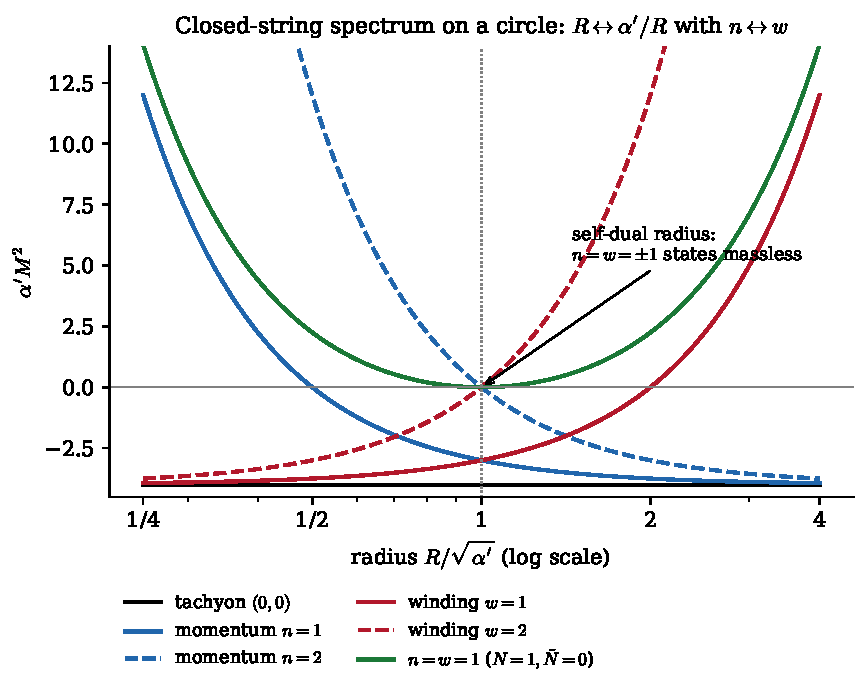
\includegraphics[width=\linewidth]{circle_spectrum.pdf}
\caption{Lowest mass levels of the closed bosonic string on a circle of radius $R$ as a function of $\log R$, with the lowest oscillator levels allowed by level matching $N-\tilde N=nw$. Momentum and winding curves are mirror images under $R\mapsto\alpha'/R$; at the self-dual radius the $n=w=\pm1$ states become massless (enhanced gauge symmetry). \emph{Computed figure; data: Tong \S{}8.2, ll. 11351--11470; Lean \texttt{leftMomentum}, \texttt{rightMomentum} (units $\alpha'$ = 1).}}
\label{fig:circle_spectrum}
\end{figure}
% [/fig:circle_spectrum]
% [fig:narain_lattice_circle] generated by tools/insert_paper_figures.py from tools/book_figures.py
\begin{figure}[tbp]
\centering
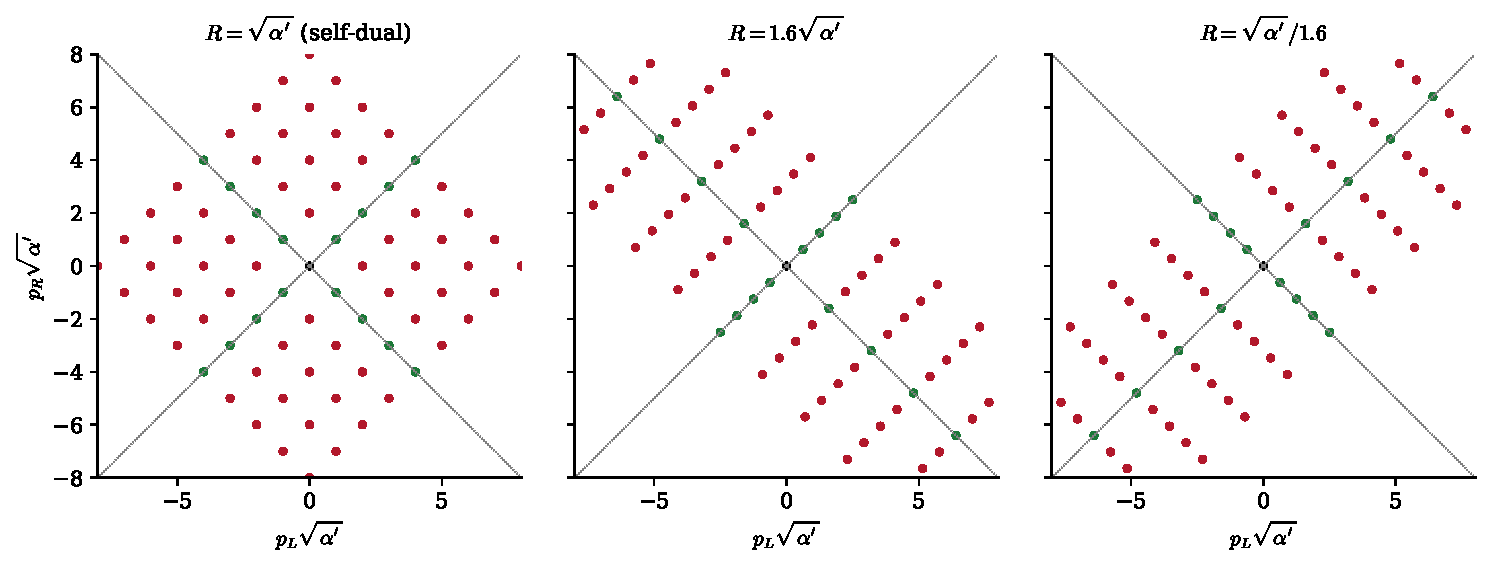
\includegraphics[width=\linewidth]{narain_lattice_circle.pdf}
\caption{The Narain lattice $\Gamma^{1,1}$ of zero-mode momenta $(p_L,p_R)$ for $|n|,|w|\le4$ at three radii. Changing $R$ is a Lorentz boost in the $(p_L,p_R)$ plane that preserves $p_L^2-p_R^2=4nw$ (dotted light-cone lines); the lattices at $R$ and $\alpha'/R$ coincide after $p_R\mapsto-p_R$ --- T-duality. \emph{Computed figure; data: Lean \texttt{leftMomentum}, \texttt{rightMomentum}; GPR \S{}2.3; Tong \S{}8.2.}}
\label{fig:narain_lattice_circle}
\end{figure}
% [/fig:narain_lattice_circle]
\label{sec:factorized}
GPR's eq.~(2.4.29) (ll.~1399--1422) exhibits, for each circle $k$ of the torus, a \emph{factorized
duality}
$D_k=\begin{pmatrix}I-e_k & e_k\\ e_k & I-e_k\end{pmatrix}$, $e_k$ the rank-one projector onto the
$k$-th coordinate, described there as ``a generalization of the $R\to 1/R$ circle duality in the
$X^i$ direction.'' \texttt{TDuality.Factorized} proves each $D_k\in O(d,d;\mathbb{Z})$
(\texttt{factorized\_isODD}), an involution (\texttt{factorized\_mul\_self}), and that distinct
$D_k,D_l$ commute (\texttt{factorized\_comm}); on $T^2$, $D_0D_1=\eta$, dualizing both circles
recovers the full duality (\texttt{factorized\_two}). The charge norm $Z^{\mathsf T}\eta Z=2\,n\cdot w$
for $Z=(n,w)$ (\texttt{chargeNorm\_sumElim}) is always even, i.e.\ $\Gamma^{d,d}$ is an even
lattice generalizing Stream~1's rank-1 statement (\texttt{chargeNorm\_even}), and is invariant
under every element of $O(d,d;\mathbb{Z})$, not merely the generators
(\texttt{chargeNorm\_invariant}).

A stronger structural fact, \emph{spectrum equivalence} (\texttt{TDuality.Spectrum}), goes beyond
the generators: every $g\in O(d,d;\mathbb{Z})$ is invertible over $\mathbb{Z}$ with inverse
$\eta g^{\mathsf T}\eta$, itself in $O(d,d;\mathbb{Z})$ (\texttt{isODD\_left\_inv/\_right\_inv/\_inv\_isODD}).
Consequently, for \emph{any} real background $H$ and \emph{any} $g\in O(d,d;\mathbb{Z})$, there is
an explicit bijection $e$ of the integer charge lattice (namely $Z\mapsto g\cdot Z$, with inverse
$Z\mapsto \eta g^{\mathsf T}\eta\cdot Z$) under which the mass form and charge norm of the
dual background $g^{\mathsf T}Hg$ at $Z$ equal those of $H$ at $e(Z)$
(\texttt{spectrum\_equivalence}). This is a charge-by-charge matching of the discrete
(mass$^2$, level) data of two $O(d,d;\mathbb{Z})$-related backgrounds; GPR's statement that the
\emph{full} partition function (with its oscillator sums and modular integral) is invariant
(l.~1417) is a strictly stronger claim, Tier~L, and is not what is proved here.

\subsection{Mirror symmetry on $T^2$}
On $T^2$, GPR remark (l.~344) that for a complex torus ``mirror symmetry is identical to what is
called `factorized duality'.'' \texttt{TDuality.Mirror} verifies the exact integer identity, first
checked with sympy (\tierS),
\begin{equation}
  D_0\cdot\operatorname{diag}(T,(T^{\mathsf T})^{-1})\cdot D_0 = g_\Theta^{\mathsf T},\qquad
  T=\begin{pmatrix}1&1\\0&1\end{pmatrix},\ \Theta=\begin{pmatrix}0&-1\\1&0\end{pmatrix},
\end{equation}
i.e.\ the factorized duality conjugates the unimodular basis change $T$ (the $\tau\mapsto\tau+1$
generator acting on the complex-structure modulus) into the transpose of an antisymmetric
$\Theta$-shift (\texttt{mirror\_conjugates\_tauShift}), which by \Cref{sec:dft}'s
\texttt{DFT.BShift.genMetric\_bshift} is exactly the form that shifts the generalized metric's
$B$-field integrally. This is the algebraic content behind ``factorized duality exchanges the
complex-structure and K\"ahler moduli of $T^2$''; which \emph{sign} of the induced $\rho$-shift
this corresponds to is a convention-dependent orientation choice for $\rho=B+i\sqrt{\det G}$ and
is not claimed.

\subsection{$SL(2,\mathbb{Z})\times SL(2,\mathbb{Z})$ at $d=2$}
% [fig:modular_fundamental_domain] generated by tools/insert_paper_figures.py from tools/book_figures.py
\begin{figure}[tbp]
\centering
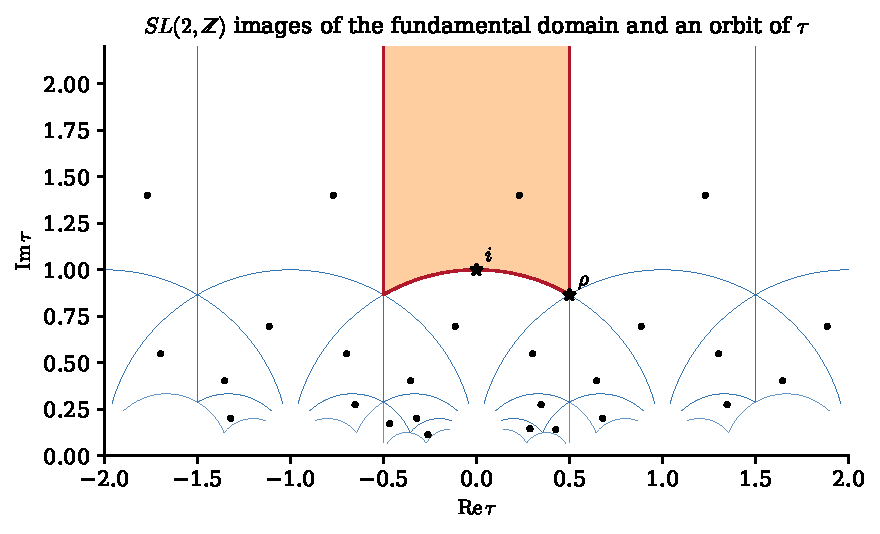
\includegraphics[width=\linewidth]{modular_fundamental_domain.pdf}
\caption{The standard fundamental domain of $SL(2,\mathbb{Z})$ (shaded) and its images under words of length $\le4$ in $S:\tau\mapsto-1/\tau$ and $T:\tau\mapsto\tau+1$, together with the orbit of one point. For $T^2$ the same picture holds for both moduli $\tau$ and $\rho$, exchanged by mirror symmetry. \emph{Computed figure; data: GPR \S{}2.5 / Tong \S{}6 (modular group); Lean \texttt{tauShift}, \texttt{mirror\_conjugates\_tauShift}.}}
\label{fig:modular_fundamental_domain}
\end{figure}
% [/fig:modular_fundamental_domain]
GPR's ``The $d=2$ Example'' (ll.~1874--1884) states that the full $T^2$ duality group is
$SL(2,\mathbb{Z})_\tau\times SL(2,\mathbb{Z})_\rho\otimes_S[\mathbb{Z}_2\times\mathbb{Z}_2]$ ---
explicitly \emph{not} a naive factorization of $O(2,2;\mathbb{Z})$. \texttt{TDuality.SL2Product}
formalizes a deliberately narrower slice: with $J=\begin{pmatrix}0&1\\-1&0\end{pmatrix}$, the
identity $AJA^{\mathsf T}=\det(A)\cdot J$ for every $2\times2$ integer $A$
(\texttt{mul\_jMat\_mul\_transpose}, sympy-checked first, \tierS, then proved by \texttt{ring} in
Lean, so this one \emph{is} Tier~A as stated), together with the monoid law for basis changes
(\texttt{basisChange\_mul}) and the additive group law for $\Theta$-shifts
(\texttt{thetaShift\_mul}). The headline result,
\texttt{basisChange\_comm\_thetaShift}, proves that a basis change with $\det A=1$ commutes with
every $\rho$-translation $g_{tJ}$ (an integer $\Theta$-shift along $J$). \textbf{Only this
direction is proved}; the converse --- that the commutator is nonzero when $\det A\ne1$ --- was
checked symbolically with sympy during development and is explicitly \emph{not} a Lean theorem
(\tierS): it must not be read as Tier~A. Consequently what is certified is that
$SL(2,\mathbb{Z})_\tau$ and the $\rho$-translations generate a commuting product inside
$O(2,2;\mathbb{Z})$; the $\rho\mapsto-1/\rho$ generator and the full $SL(2,\mathbb{Z})_\rho$ are
not formalized.

\begin{table}[htbp]
\centering\footnotesize
\caption{T-duality layer: Lean declaration and epistemic tier.}
\label{tab:tduality}
\begin{tabular}{@{}l l@{}}
\toprule
\textbf{Lean declaration} & \textbf{Tier / content} \\ \midrule
\texttt{thetaShift\_isODD} & A --- $\Theta^{\mathsf T}=-\Theta \Rightarrow g_\Theta\in O(d,d;\mathbb{Z})$ (one direction) \\
\texttt{basisChange\_isODD} & A --- $A^{\mathsf T}B=1\Rightarrow\operatorname{diag}(A,B)\in O(d,d;\mathbb{Z})$ \\
\texttt{eta\_mul\_self/\_isODD}, \texttt{isODD\_mul} & A --- $\eta$ involutive $\in O(d,d;\mathbb{Z})$; closure \\
\texttt{eta\_one\_reindex} & A --- $d=1$: $\eta$ = Stream 1's Narain Gram matrix \\
Generators generate all of $O(d,d;\mathbb{Z})$ & L --- GPR l.~1422, not proved here \\
\texttt{factorized\_isODD/\_mul\_self/\_comm/\_two} & A --- $D_k\in O(d,d;\mathbb{Z})$, involutions, commute, $D_0D_1=\eta$ \\
\texttt{chargeNorm\_even/\_invariant} & A --- $Z^{\mathsf T}\eta Z$ even, $O(d,d;\mathbb{Z})$-invariant \\
\texttt{isODD\_left\_inv/\_right\_inv/\_inv\_isODD} & A --- every $g\in O(d,d;\mathbb{Z})$ invertible, inverse $\eta g^{\mathsf T}\eta$ \\
\texttt{spectrum\_equivalence} & A --- charge-by-charge (mass$^2$, level) matching under any $g$ \\
Full partition function invariance & L --- GPR l.~1417, strictly stronger, not proved \\
\texttt{mirror\_conjugates\_tauShift} & A --- exact matrix identity (sympy-checked convention, \tierS, before formalization) \\
Factorized duality = mirror symmetry & L --- GPR l.~344 \\
\texttt{mul\_jMat\_mul\_transpose} & A --- $AJA^{\mathsf T}=\det(A)J$ \\
\texttt{basisChange\_comm\_thetaShift} & A --- $\det A=1\Rightarrow$ commutes with $\rho$-translations (one direction) \\
Converse ($\det A\ne1\Rightarrow$ noncommuting) & \tierS\ --- sympy only, not a Lean theorem \\
Full $SL(2,\mathbb{Z})_\tau\times SL(2,\mathbb{Z})_\rho$ & L --- GPR ll.~1874--1884, not claimed \\
\bottomrule
\end{tabular}
\end{table}

%%%%%%%%%%%%%%%%%%%%%%%%%%%%%%%%%%%%%%%%%%%%%%%%%%%%%%%%%%%%%%%%%%%%%%%%%%%%%%%
\section{Double Field Theory}
\label{sec:dft}
%%%%%%%%%%%%%%%%%%%%%%%%%%%%%%%%%%%%%%%%%%%%%%%%%%%%%%%%%%%%%%%%%%%%%%%%%%%%%%%

\subsection{The generalized metric}
Hull and Zwiebach's Double Field Theory packages the torus metric $G$ and Kalb--Ramond field $B$
into a single object valued in the coset $O(d,d)/(O(d)\times O(d))$, the \emph{generalized metric}
(arXiv:0904.4664, eq.~(2.17), ll.~662--672)
\begin{equation}
  \mathcal{H}(G,B) = \begin{pmatrix} G - BG^{-1}B & BG^{-1} \\ -G^{-1}B & G^{-1}\end{pmatrix},
  \qquad \mathcal{H}^{-1}=\eta\mathcal{H}\eta.
\end{equation}
\texttt{DFT.GeneralizedMetric} proves, over $\mathbb{R}$ for every $d$, the constraint in the form
$(\eta\mathcal{H})^2=1$ (\texttt{etaR\_genMetric\_sq}) requiring \emph{only} that $G$ be invertible
--- neither symmetry of $G$ nor antisymmetry of $B$ is used in this proof, which is sharper than
Hull--Zwiebach's own statement (stated there for the physical $G,B$). Symmetry of $\mathcal{H}$
under the physical hypotheses $G^{\mathsf T}=G$, $B^{\mathsf T}=-B$ is proved separately
(\texttt{genMetric\_symm}). At $B=0$, conjugating by the full duality inverts the metric,
$\eta\,\mathcal{H}(G,0)\,\eta=\mathcal{H}(G^{-1},0)$ (\texttt{tduality\_inverts\_metric}): T-duality
\emph{is} the map $G\mapsto G^{-1}$ at the level of the generalized metric. The mass form
$Z^{\mathsf T}\mathcal{H}Z$ is covariant under \emph{any} matrix $g$ (again no $O(d,d)$ hypothesis
is needed for this identity: $\mathrm{massForm}(g^{\mathsf T}Hg,Z)=\mathrm{massForm}(H,gZ)$,
\texttt{massForm\_covariant}), which is what makes the spectrum-equivalence argument of
\Cref{sec:tduality} work once $g\in O(d,d;\mathbb{Z})$ is assumed there. On a circle ($d=1$,
$G=R^2$, $B=0$), \texttt{massForm\_circle} proves the DFT mass form equals exactly one half of
Stream~1's $P_L^2+P_R^2=\mathtt{momentumMassSq}$ --- so Stream~2's general-$d$ DFT layer and
Stream~1's original circle computation are proved identical at $d=1$, not merely analogous.

\subsection{$B$-field shifts}
% [fig:generalized_metric_odd] generated by tools/insert_paper_figures.py from tools/book_figures.py
\begin{figure}[tbp]
\centering
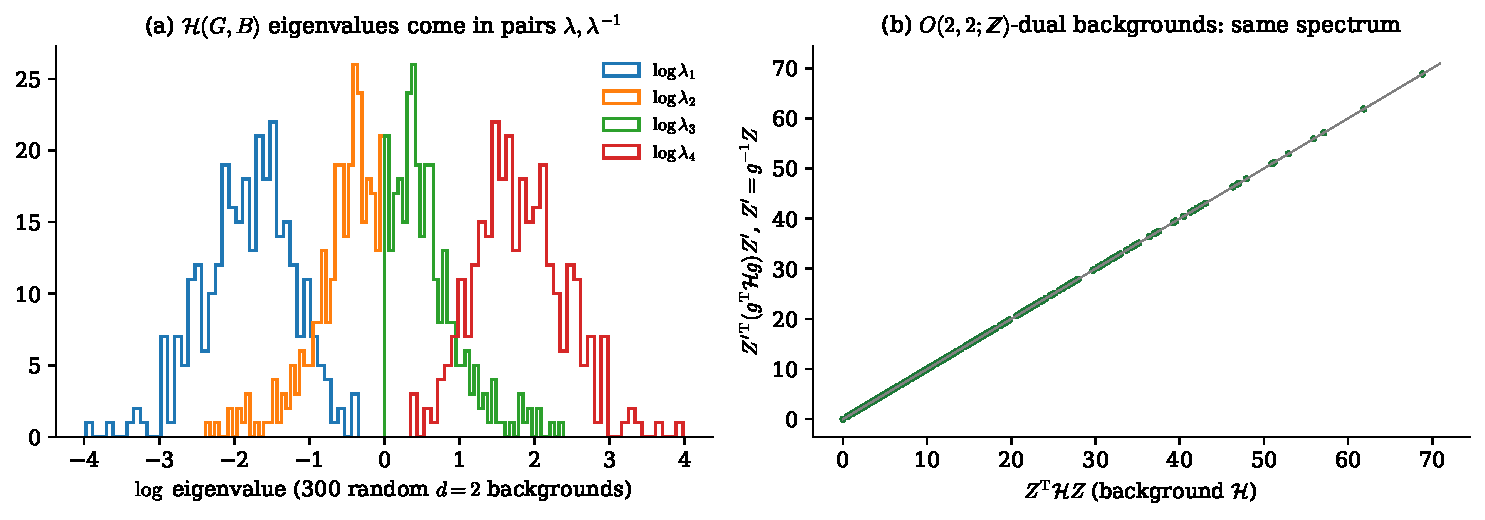
\includegraphics[width=\linewidth]{generalized_metric_odd.pdf}
\caption{(a) Logarithms of the four eigenvalues of the generalized metric $\mathcal{H}(G,B)$ for 300 random backgrounds on $T^2$: they are symmetric about $0$, because $(\eta\mathcal{H})^2=1$ (\texttt{etaR\_genMetric\_sq}) forces eigenvalues in pairs $\lambda,\lambda^{-1}$. (b) For $g=\Theta\cdot A\cdot\text{(factorized duality)}\cdot\Theta'\in O(2,2;\mathbb{Z})$, the mass form of every charge $Z$ in background $\mathcal{H}$ equals that of $g^{-1}Z$ in the dual background $g^{\mathrm{T}}\mathcal{H}g$: the points lie on the diagonal (\texttt{spectrum\_equivalence}, \texttt{massForm\_covariant}). \emph{Computed figure; data: Lean \texttt{genMetric} (GeneralizedMetric.lean), \texttt{thetaShift}, \texttt{basisChange}, \texttt{factorized}; HHZ \S{}2.}}
\label{fig:generalized_metric_odd}
\end{figure}
% [/fig:generalized_metric_odd]
GPR's remark that the $\Theta$-shift ``gives only topological contributions'' to the spectrum
(eq.~(2.4.25) context) is realized at the level of the generalized metric: for invertible
symmetric $G$ and antisymmetric $B,\Theta$,
\begin{equation}
  g_\Theta\cdot\mathcal{H}(G,B)\cdot g_\Theta^{\mathsf T} = \mathcal{H}(G,\,B+\Theta)
  \qquad(\texttt{genMetric\_bshift}),
\end{equation}
so the periodic identification $B\sim B+\Theta$ is exactly an $O(d,d;\mathbb{Z})$ duality of the
DFT background (combined with \texttt{TDuality.thetaShift\_isODD}, the real $\Theta$-shift also preserves
$\eta$: \texttt{thetaShiftR\_preserves\_eta}). Shifting by $\Theta$ and then by $-\Theta$ returns
the original background (\texttt{genMetric\_bshift\_cancel}). The overall sign/transpose
convention in the formula above was checked with sympy \emph{before} the Lean statement was
written (\tierS): of four candidate placements of $\pm\Theta$ and transposes, exactly this one
holds; the Lean theorem is the resulting Tier~A statement, not the sympy check itself.

\subsection{Level matching and the section condition}
Hull--Zwiebach's level-matching condition, $L_0-\bar L_0=N-\bar N-p_a w^a=0$ (eq.~(1.3), l.~231),
at equal oscillator number $N=\bar N$ reduces to $n\cdot w=0$, i.e.\ the charge is $\eta$-null.
\texttt{DFT.SectionCondition} proves this equivalence exactly
(\texttt{levelMatching\_iff}: $\mathrm{chargeNorm}(n,w)=0 \iff n\cdot w=0$). A set of charges is a
\emph{section} if it is totally $\eta$-null (\texttt{IsSection}); Hull--Zwiebach's description of
the two extreme solutions of the strong section condition --- ``independent of $\tilde x$'' (the
ordinary supergravity fields) and ``independent of $x^a$'' (their duals), ll.~339--342, and
``totally null $d$-dimensional subspaces,'' ll.~3930--3940 --- correspond here to the pure-momentum
frame and the pure-winding frame, each proved to be a section
(\texttt{momentumFrame\_isSection}, \texttt{windingFrame\_isSection}). The full duality $\eta$ maps
the momentum frame onto the winding frame (\texttt{eta\_momentum\_to\_winding}), and any
$g\in O(d,d;\mathbb{Z})$ maps sections to sections (\texttt{isSection\_image}) --- the section
condition is preserved along the whole duality orbit, not merely at the two frames exhibited by
name.

\begin{table}[htbp]
\centering\footnotesize
\caption{Double Field Theory layer: Lean declaration and epistemic tier.}
\label{tab:dft}
\begin{tabular}{@{}l l@{}}
\toprule
\textbf{Lean declaration} & \textbf{Tier / content} \\ \midrule
\texttt{etaR\_genMetric\_sq} & A --- $(\eta\mathcal{H})^2=1$ for any invertible $G$ (sharper than HZ) \\
\texttt{genMetric\_symm} & A --- $\mathcal{H}$ symmetric for $G$ symm., $B$ antisymm. \\
\texttt{tduality\_inverts\_metric} & A --- $\eta\mathcal{H}(G,0)\eta=\mathcal{H}(G^{-1},0)$ \\
\texttt{massForm\_covariant} & A --- covariance under \emph{any} $g$ (no $O(d,d)$ hypothesis) \\
\texttt{massForm\_circle} & A --- $d=1$ DFT mass form = $\tfrac12\times$ Stream 1's \texttt{momentumMassSq} \\
\texttt{genMetric\_bshift} & A --- $g_\Theta\mathcal{H}(G,B)g_\Theta^{\mathsf T}=\mathcal{H}(G,B+\Theta)$ \\
Sign/transpose convention & \tierS\ --- sympy, checked before formalization \\
\texttt{thetaShiftR\_preserves\_eta}, \texttt{genMetric\_bshift\_cancel} & A --- real $\Theta$-shift $\in O(d,d)$; shift-and-unshift \\
\texttt{levelMatching\_iff} & A --- $L_0=\bar L_0 \iff n\cdot w=0$ \\
\texttt{momentumFrame\_isSection}, \texttt{windingFrame\_isSection} & A --- pure-momentum/-winding frames are sections \\
\texttt{eta\_momentum\_to\_winding}, \texttt{isSection\_image} & A --- $\eta$ swaps frames; $O(d,d;\mathbb{Z})$ preserves sections \\
\bottomrule
\end{tabular}
\end{table}

%%%%%%%%%%%%%%%%%%%%%%%%%%%%%%%%%%%%%%%%%%%%%%%%%%%%%%%%%%%%%%%%%%%%%%%%%%%%%%%
\section{The dual-scale trace bound}
% [fig:dual_scale_bound] generated by tools/insert_paper_figures.py from tools/book_figures.py
\begin{figure}[tbp]
\centering
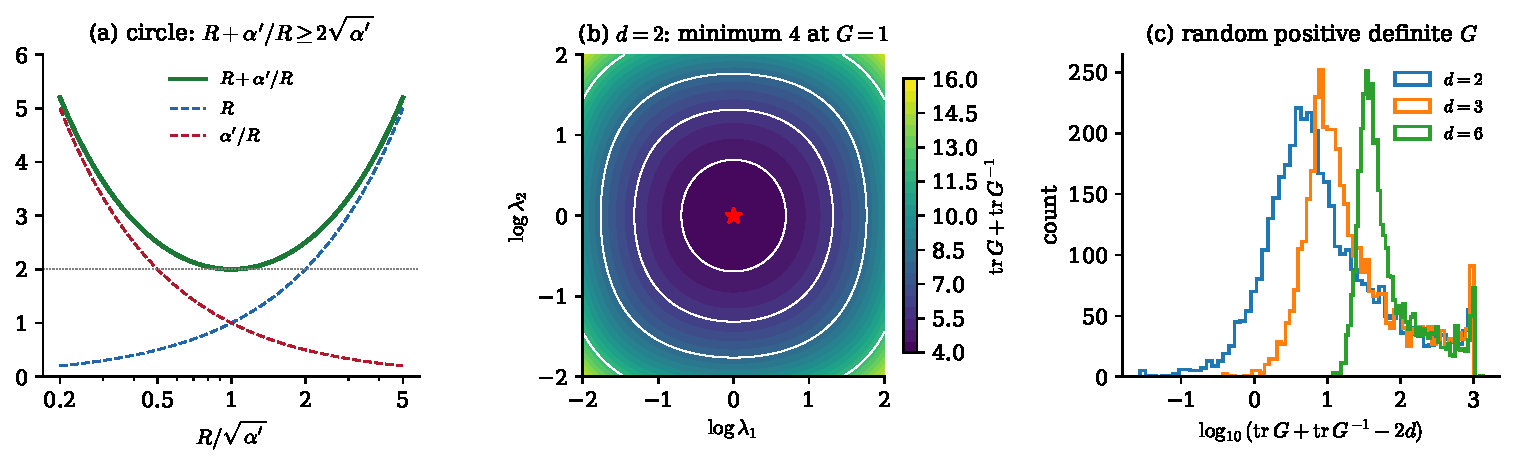
\includegraphics[width=\linewidth]{dual_scale_bound.pdf}
\caption{The dual-scale bound. (a) On a circle the effective scale $R+\alpha'/R$ is minimized at the self-dual radius. (b) For $d=2$ and positive-definite $G$ with eigenvalues $\lambda_{1,2}$, $\mathrm{tr}\,G+\mathrm{tr}\,G^{-1}=\sum_i(\lambda_i+\lambda_i^{-1})$ has its minimum $2d=4$ at $G=1$. (c) Excess over $2d$ for 4000 random positive definite matrices in each dimension: never negative, as the Lean theorem \texttt{dualScale\_ge} guarantees. The plot illustrates the theorem; it proves nothing. \emph{Computed figure; data: Lean \texttt{dualScale\_circle}, \texttt{circle\_effective\_scale\_ge\_two}, \texttt{dualScale\_ge} (TraceBound.lean).}}
\label{fig:dual_scale_bound}
\end{figure}
% [/fig:dual_scale_bound]
\label{sec:trace-bound}
%%%%%%%%%%%%%%%%%%%%%%%%%%%%%%%%%%%%%%%%%%%%%%%%%%%%%%%%%%%%%%%%%%%%%%%%%%%%%%%

This research programme's recurring proposal (Stream~1,
\texttt{DualScaleM24Formalization.DualScale.EffectiveMetric.genesis\_no\_singularity}, and paper~7's
``The Effective Dual Scale and Singularity Resolution'' section) is the one-dimensional statement that the effective scale probed by a
string, $R_{\mathrm{eff}}(R)=R+\alpha'/R$, is bounded below by $2\sqrt{\alpha'}$, attained at the
self-dual radius. \texttt{DualScale.TraceBound} generalizes this to every flat torus metric
$G$ (a positive-definite $d\times d$ real matrix), defining the \emph{dual scale} as the trace of
the generalized metric at $B=0$:
\begin{equation}
  \mathcal{D}(G) \;:=\; \operatorname{tr}\mathcal{H}(G,0) \;=\; \operatorname{tr}G + \operatorname{tr}G^{-1}
  \qquad (\texttt{dualScale\_eq}).
\end{equation}
This is invariant under the full T-duality, $\mathcal{D}(G^{-1})=\mathcal{D}(G)$
(\texttt{dualScale\_inv}), and satisfies, for every positive-definite $G$,
\begin{equation}
  \mathcal{D}(G) \;\ge\; 2d \qquad (\texttt{dualScale\_ge}),
\end{equation}
proved directly from $\operatorname{tr}\big((G-1)^{\mathsf T}G^{-1}(G-1)\big)\ge 0$ (positive
semi-definiteness of a conjugate of a positive-definite matrix), which expands to
$\operatorname{tr}G+\operatorname{tr}G^{-1}-2d\ge0$ --- \emph{no eigenvalue decomposition of $G$
is used}. The bound is attained at the self-dual metric $G=\mathbf 1_d$,
$\mathcal{D}(\mathbf 1_d)=2d$ (\texttt{dualScale\_one}), \textbf{and only there}: for
positive-definite $G$,
\begin{equation}
  \mathcal{D}(G)=2d \iff G=\mathbf 1_d \qquad(\texttt{dualScale\_eq\_iff}).
\end{equation}
The first version of this paper proved attainment only and declined to write ``equality iff''; the
uniqueness half was added in Revision~2. Its proof: equality forces
$\operatorname{tr}\big((G-1)^{\mathsf T}G^{-1}(G-1)\big)=0$; a positive-semidefinite matrix with zero
trace is zero (Mathlib's \texttt{PosSemidef.trace\_eq\_zero\_iff}, which rests on the spectral
theorem --- so, unlike \texttt{dualScale\_ge}, this half does use eigenvalues, inside Mathlib); and
since $G^{-1}$ is positive \emph{definite}, $x^{\mathsf T}(G-1)^{\mathsf T}G^{-1}(G-1)x=0$ for all $x$
forces $G=\mathbf 1_d$. This is a statement at $B=0$; nothing is proved about the minimizer once
$B\ne0$. At $d=1$, $G=R^2$,
\begin{equation}
  \mathcal{D}(R^2) = (R+R^{-1})^2-2 \qquad(\texttt{dualScale\_circle}),
\end{equation}
and specializing \texttt{dualScale\_ge} to $d=1$ together with this identity gives exactly
\begin{equation}
  R + R^{-1} \ge 2 \qquad \text{for all } R>0 \qquad (\texttt{circle\_effective\_scale\_ge\_two}),
\end{equation}
the real-number form of the one-dimensional dual-scale bound, now proved over $\mathbb{R}$ (using
Mathlib) rather than only the $\mathbb{N}$-instance available to the Mathlib-free Stream~1 corpus.

\paragraph{Physical reading (Tier~C).} At the self-dual point $G=\mathbf 1_d$ the trace bound is
saturated: reading $\mathcal{D}(G)$ as a proxy for an effective probed length scale, no
$O(d,d;\mathbb{Z})$-invariant combination of the torus radii can be driven below this value by any
sequence of T-dualities. As in paper~7, we flag this as exactly the same kind of \emph{kinematic}
statement as the circle case: a bound on a specific algebraic quantity built from the metric, not
a dynamical proof that any cosmological evolution of $G(t)$ must bounce through this regime, and
not a proof of a minimum \emph{physical} length in any operational sense. Any singularity-resolution
or minimum-length reading of this bound remains Tier~C, exactly as it was for the $d=1$ statement
in Stream~1 and paper~7.

\begin{table}[htbp]
\centering\footnotesize
\caption{Dual-scale bound: Lean declaration and epistemic tier.}
\label{tab:tracebound}
\begin{tabular}{@{}l l@{}}
\toprule
\textbf{Lean declaration} & \textbf{Tier / content} \\ \midrule
\texttt{dualScale\_eq} & A --- $\mathcal{D}(G)=\operatorname{tr}G+\operatorname{tr}G^{-1}$ \\
\texttt{dualScale\_inv} & A --- $\mathcal{D}(G^{-1})=\mathcal{D}(G)$ \\
\texttt{dualScale\_ge} & A --- $\mathcal{D}(G)\ge 2d$ for $G$ positive definite \\
\texttt{dualScale\_one} & A --- bound attained at $G=\mathbf 1_d$ \\
\texttt{dualScale\_eq\_iff} & A --- $\mathcal{D}(G)=2d\iff G=\mathbf 1_d$, $G$ pos.\ def.\ (Rev.~2) \\
\texttt{dualScale\_circle} & A --- $d=1$: $\mathcal{D}(R^2)=(R+R^{-1})^2-2$ \\
\texttt{circle\_effective\_scale\_ge\_two} & A --- $R+R^{-1}\ge2$, real, for all $R>0$ \\
Singularity resolution / minimum length & C --- physical reading, not proved \\
\bottomrule
\end{tabular}
\end{table}

%%%%%%%%%%%%%%%%%%%%%%%%%%%%%%%%%%%%%%%%%%%%%%%%%%%%%%%%%%%%%%%%%%%%%%%%%%%%%%%
\section{Flux and tadpole cancellation on $K3\times T^2$ and $K3\times K3$}
% [fig:tadpole_budget] generated by tools/insert_paper_figures.py from tools/book_figures.py
\begin{figure}[tbp]
\centering
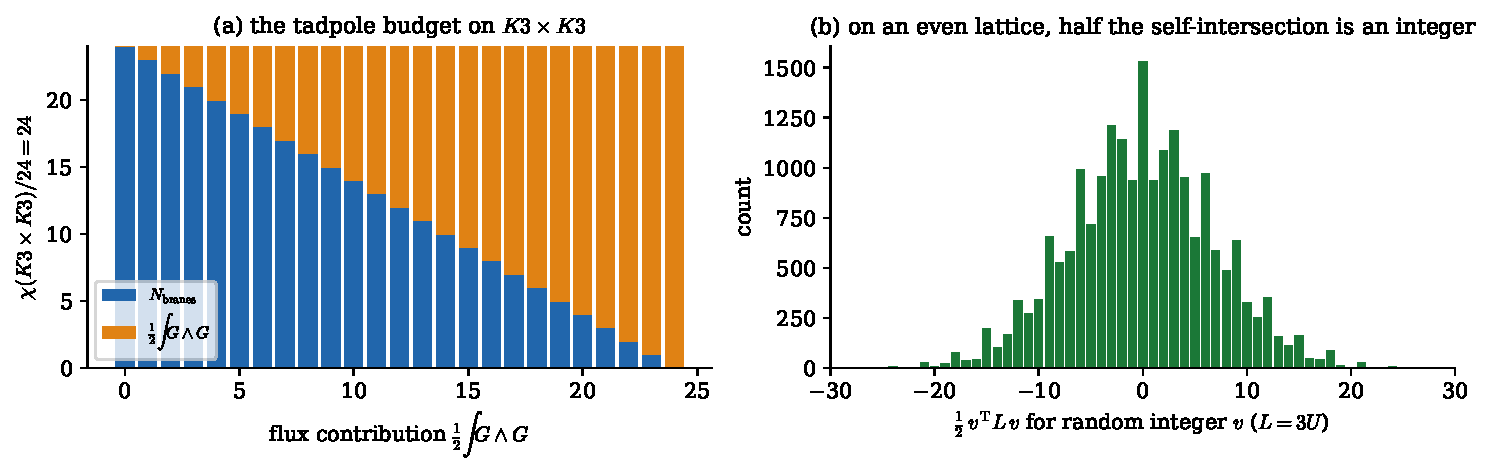
\includegraphics[width=\linewidth]{tadpole_budget.pdf}
\caption{(a) Every way to split the tadpole budget $\chi(K3\times K3)/24=576/24=24$ between space-filling branes and flux (\texttt{k3k3\_anomaly}, \texttt{tadpole\_budget}). (b) For random integer flux vectors on the even lattice $3U$, $\frac12 v^{\mathrm{T}}Lv$ is always an integer, the lattice fact behind flux quantization (\texttt{kronForm\_even}, \texttt{flux\_half\_selfIntersection\_integral}). \emph{Computed figure; data: SVW ($\chi$/24 condition); DRS \S{}2--4; Lean Flux/Tadpole.lean, Flux/Integrality.lean.}}
\label{fig:tadpole_budget}
\end{figure}
% [/fig:tadpole_budget]
\label{sec:flux}
%%%%%%%%%%%%%%%%%%%%%%%%%%%%%%%%%%%%%%%%%%%%%%%%%%%%%%%%%%%%%%%%%%%%%%%%%%%%%%%

Dasgupta, Rajesh, and Sethi study M-theory and type~IIB orientifold compactifications on
$K3\times T^2$/$K3\times K3$ with G-flux (hep-th/9908088) \cite{DasguptaRajeshSethi1999}. For
M-theory on $K3\times K3$, ``the anomaly $\chi/24=24$ ... must be cancelled by a combination of
branes and G-flux'' (\S3.1, l.~640); the type~IIB orientifold of $K3\times T^2$ is the F-theory
dual of that setup (ll.~1265ff), with tadpole condition $\tfrac12\int(G/2\pi)\wedge(G/2\pi)+n=24$
(ll.~1366--1370), and with no flux, ``type~I on $K3\times T^2$ with 24 D5-branes'' (l.~1275).

\texttt{Flux.Tadpole} computes Euler characteristics from Hodge-number tables via
$\chi=\sum_{p,q}(-1)^{p+q}h^{p,q}$ (\texttt{eulerFromHodge}), reusing Stream~1's certified $K3$
Hodge diamond (\texttt{StringTheoryFormalization.Frontier.HodgeNumbers.k3HodgeNumber}) rather than
re-tabulating it: $\chi(T^2)=0$ (\texttt{euler\_T2}) and $\chi(K3)=24$ (\texttt{euler\_K3}). By
K\"unneth (Tier~L; not separately formalized here), $\chi(K3\times K3)=\chi(K3)^2$
(\texttt{chiK3K3}), giving $\chi(K3\times K3)/24=24$ exactly, an integer
(\texttt{k3k3\_anomaly}), matching DRS's stated anomaly value. Separately,
$\chi(K3)\cdot\chi(T^2)=0$ (\texttt{k3t2\_euler\_zero}): $K3\times T^2$ itself contributes no
curvature tadpole, consistent with the flux/brane budget being the only source of the anomaly
there. The D3/flux budget arithmetic $\mathrm{flux}+n=24$, $\mathrm{flux}\ge0
\Rightarrow n\le24$, and $\mathrm{flux}=0\Rightarrow n=24$ (\texttt{tadpole\_budget}) is a direct
consequence of the stated tadpole condition; nothing about the \emph{existence} of a
flux configuration achieving any particular budget is claimed.

Why the flux contribution is an integer in the first place is a separate fact, proved in
\texttt{Flux.Integrality}: DRS's Dirac-quantization argument (ll.~230--232, ``If $\chi/24\in
\mathbb{Z}$ then $[G/2\pi]$ is an integer cohomology class'') combined with K\"unneth's
identification $H^2(K3)\otimes H^2(K3)\subset H^4(K3\times K3)$ (both Tier~L) reduces the claim
$\tfrac12\int G\wedge G\in\mathbb{Z}$ to a statement about the Kronecker product of the $K3$
intersection form with itself. \texttt{Flux.Integrality} proves, for \emph{any} two symmetric
integer forms $L_1,L_2$ with $L_1$ even, that their Kronecker product $L_1\otimes L_2$ is again an
even form (\texttt{kronForm\_even}), and hence that every self-intersection
$x^{\mathsf T}(L_1\otimes L_2)x$ is exactly twice an integer
(\texttt{flux\_half\_selfIntersection\_integral}: $\exists k,\ x^{\mathsf T}(L_1\otimes L_2)x=2k$).
Since the $K3$ lattice's summands $U$ and $E_8(-1)$ are already proved even
(\Cref{sec:lattices}), this instantiates to flux forms $G\in H^2(K3)\otimes H^2(K3)$. The Lean
theorem is purely about the Kronecker product of two abstract integer forms; the identification of
$G$ with a flux configuration and of $x^{\mathsf T}(L_1\otimes L_2)x$ with $\int G\wedge G$ is the
K\"unneth/Dirac-quantization input, Tier~L. Gukov--Vafa--Witten's superpotential for flux
compactifications on Calabi--Yau fourfolds \cite{GukovVafaWitten1999} is cited here only as
context for why flux superpotentials of this kind matter physically on $K3\times T^2$; no Lean
module in this corpus formalizes any part of the GVW superpotential itself.

\begin{table}[htbp]
\centering\footnotesize
\caption{Flux and tadpole layer: Lean declaration and epistemic tier.}
\label{tab:flux}
\begin{tabular}{@{}l l@{}}
\toprule
\textbf{Lean declaration} & \textbf{Tier / content} \\ \midrule
\texttt{euler\_T2}, \texttt{euler\_K3} & A --- $\chi(T^2)=0$, $\chi(K3)=24$ from Hodge tables \\
\texttt{k3k3\_anomaly} & A --- $\chi(K3\times K3)/24=24\in\mathbb{Z}$ (K\"unneth is L) \\
\texttt{k3t2\_euler\_zero} & A --- $\chi(K3)\chi(T^2)=0$ \\
\texttt{tadpole\_budget} & A --- arithmetic consequence of $\mathrm{flux}+n=24$ \\
Tadpole condition, DRS eqs.\ (line refs above) & L --- Dasgupta--Rajesh--Sethi \\
\texttt{kronForm\_even}, \texttt{flux\_half\_selfIntersection\_integral} & A --- even $\otimes$ any = even; self-intersections are $2k$ \\
Künneth identification with $\int G\wedge G$; Dirac quantization & L --- DRS ll.\,230--232; Künneth \\
GVW flux superpotential & L --- context only, not formalized \\
\bottomrule
\end{tabular}
\end{table}

%%%%%%%%%%%%%%%%%%%%%%%%%%%%%%%%%%%%%%%%%%%%%%%%%%%%%%%%%%%%%%%%%%%%%%%%%%%%%%%
\section{Mathieu moonshine arithmetic}
% [fig:moonshine_coefficients] generated by tools/insert_paper_figures.py from tools/book_figures.py
\begin{figure}[tbp]
\centering
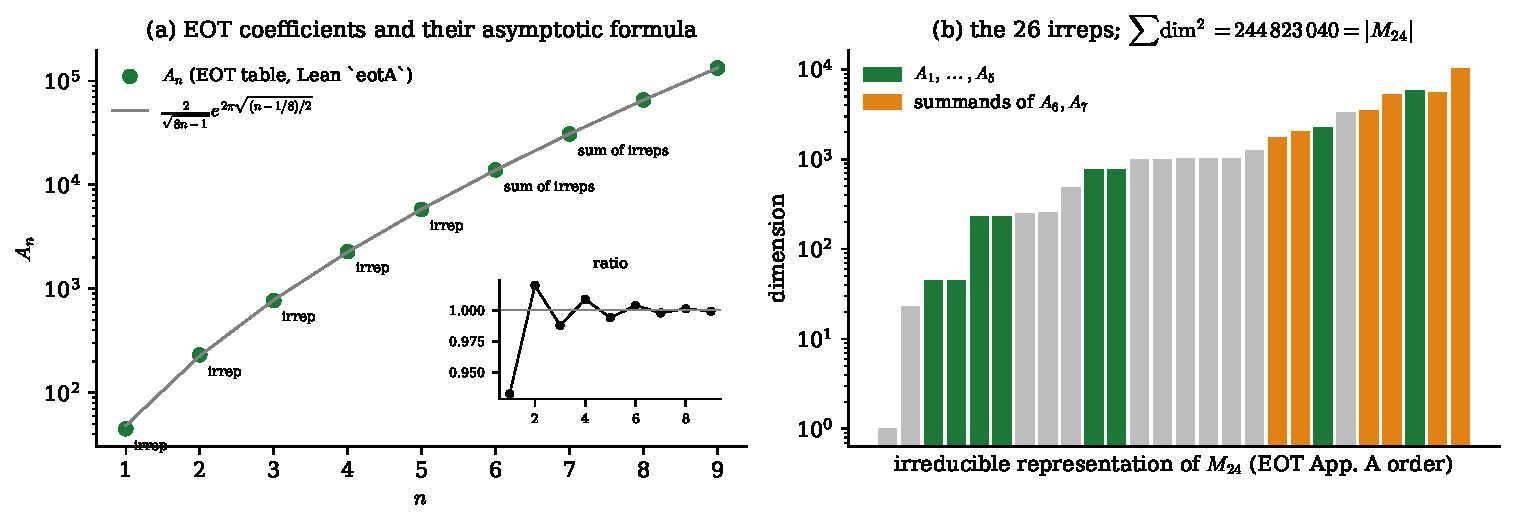
\includegraphics[width=\linewidth]{moonshine_coefficients.pdf}
\caption{(a) The coefficients $A_n$ of the K3 elliptic genus (EOT eq. 1.12, the Lean table \texttt{eotA}) against the asymptotic formula EOT eq. (1.13); the inset shows the ratio. $A_1,\dots,A_5$ are dimensions of irreducible representations of $M_{24}$; $A_6$ and $A_7$ are sums of them. (b) The 26 irreducible dimensions of $M_{24}$ from the Lean table \texttt{M24RepDim}; the sum of their squares equals the group order (\texttt{M24RepDim\_sum\_sq}), the check that caught an earlier wrong table. \emph{Computed figure; data: EOT eqs. (1.12)--(1.15), ll. 200--232 (formula read from the PDF page, the .txt garbles it); App. A (A.3).}}
\label{fig:moonshine_coefficients}
\end{figure}
% [/fig:moonshine_coefficients]
\label{sec:moonshine}
%%%%%%%%%%%%%%%%%%%%%%%%%%%%%%%%%%%%%%%%%%%%%%%%%%%%%%%%%%%%%%%%%%%%%%%%%%%%%%%

Eguchi, Ooguri, and Tachikawa (EOT) observed that the coefficients of the $\mathcal{N}=4$
superconformal character decomposition of the $K3$ elliptic genus,
\begin{equation}
  Z_{\mathrm{ell}}(K3) = 20\,\mathrm{ch}_{1/4,0} - 2\,\mathrm{ch}_{1/4,1/2}
    + 2\sum_{n\ge1} A_n\, q^{n-1/8}\,\theta_1^2/\eta^3
\end{equation}
(eq.~(1.11), ll.~175--195), with $A_n=45,231,770,2277,5796,13915,\dots$ (eq.~(1.12), l.~208), are
\emph{dimensions of irreducible representations} of the sporadic Mathieu group $M_{24}$ for the
first five values (ll.~227--233), a phenomenon subsequently proved in full by Gannon
\cite{Gannon2016}. \textbf{Notational note}: papers~2 and~7 of this project's own corpus use the
symbol $A_n$ for \emph{twice} EOT's coefficients (their $\mathcal{A}_n:=2A_n^{\mathrm{EOT}}$, so
that, e.g., $\mathcal{A}_1=90=\mathbf{45}\oplus\overline{\mathbf{45}}$); \texttt{Moonshine.EOT}
uses EOT's own, undoubled convention, $\mathtt{eotA}=(45,231,770,2277,5796,13915,30843,65550,132825)$
matching eq.~(1.12) directly, and this paper follows \texttt{Moonshine.EOT}'s convention
throughout this section to avoid re-introducing the ambiguity flagged in the revision brief.
Also for the record, since an earlier revision of paper~7 stated it incorrectly: EOT's eq.~(A.3)
(ll.~346--349) lists the irreducible dimensions $45,231,770,990,1035,\dots$ as coming in
complex-conjugate pairs, while $2277$ is a \emph{real} irreducible dimension, so the doubled
multiplicity is $4554=2\cdot2277$, two copies of the same real representation, not
$2277\oplus\overline{2277}$.

\texttt{Moonshine.EOT} checks the EOT arithmetic against Stream~1's own $M_{24}$ irreducible
dimension table, \texttt{StringTheory.StringDynamics.MathieuM24.M24RepDim} (itself guarded by the
Burnside identity $\sum_i \dim(i)^2=|M_{24}|=244{,}823{,}040$ in
\texttt{M24RepDim\_sum\_sq}, a Stream~1 theorem, cited here as the safeguard that this table is
correct and not, as an earlier version of it briefly was, wrong by a duplicated and a missing
entry). \texttt{first\_five\_are\_irreps} proves that each of $A_1,\dots,A_5$ equals some entry of
\texttt{M24RepDim} (witnesses at table indices $2,4,9,19,23$ for $45,231,770,2277,5796$
respectively); this is an equality against Stream~1's table, so its physical content --- that
these table entries really are $M_{24}$'s irreducible dimensions --- rests on that table's Tier~L
sourcing (EOT eq.~(A.3)) via Stream~1, not re-derived here. \texttt{A6\_decomposition} proves EOT's
eq.~(1.14), $A_6=13915=3520+10395$ (table indices 21, 25), and \texttt{A7\_decomposition} proves
eq.~(1.15), $A_7=30843=10395+5796+5544+5313+2024+1771$ (indices 25,23,24,22,18,17); both by
\texttt{rfl} on the now-corrected table. \texttt{A6\_not\_irrep} confirms that $A_6$ itself is
\emph{not} the dimension of any single irreducible representation in the table, so a genuine
decomposition (rather than a single witness, as for $A_1,\dots,A_5$) is required for it. Throughout,
that the elliptic genus decomposition in fact carries an honest $M_{24}$ \emph{action} (rather than
this arithmetic coincidence) is the moonshine phenomenon itself --- EOT's observation, proved by
Gannon \cite{Gannon2016} --- and is Tier~L, not addressed by this arithmetic module.

\begin{table}[htbp]
\centering\footnotesize
\caption{Moonshine layer: Lean declaration and epistemic tier.}
\label{tab:moonshine}
\begin{tabular}{@{}l l@{}}
\toprule
\textbf{Lean declaration} & \textbf{Tier / content} \\ \midrule
\texttt{eotA} & def --- EOT eq.\,(1.12) coefficients, undoubled convention \\
\texttt{first\_five\_are\_irreps} & A --- $A_1,\dots,A_5$ each equal an \texttt{M24RepDim} table entry \\
\texttt{A6\_decomposition}, \texttt{A7\_decomposition} & A --- EOT eqs.\,(1.14)/(1.15) sums vs.\ table \\
\texttt{A6\_not\_irrep} & A --- $A_6$ is not a single table entry \\
\texttt{M24RepDim\_sum\_sq} & A --- Stream 1, Burnside guard $\sum\dim^2=|M_{24}|$ \\
$M_{24}$ irreducible dimensions (eq.\,A.3); $M_{24}$ action on the genus & L --- EOT; Gannon \\
\bottomrule
\end{tabular}
\end{table}

%%%%%%%%%%%%%%%%%%%%%%%%%%%%%%%%%%%%%%%%%%%%%%%%%%%%%%%%%%%%%%%%%%%%%%%%%%%%%%%
\section{What is, and is not, proved}
\label{sec:scope}
%%%%%%%%%%%%%%%%%%%%%%%%%%%%%%%%%%%%%%%%%%%%%%%%%%%%%%%%%%%%%%%%%%%%%%%%%%%%%%%

\begin{scopebox}
\textbf{Is proved (Tier A, kernel-checked, 100 theorems, 0 \texttt{sorry}, standard axioms only):}
exact integer/rational identities about explicit matrices --- unimodularity and
positive-definiteness of $E_8$ and $E_8(-1)$; evenness, unimodularity, and a signature witness for
$U$; signature and rank arithmetic for the K3, Mukai, and $K3\times T^2$ lattices, cross-checked
against an independently tabulated Hodge signature; symmetry, self-pairing, and evenness of the
Mukai pairing; that $(-2)$-vector reflections are involutive isometries, instantiated to the
simple roots of $E_8(-1)$; that specific matrix families ($\Theta$-shifts under an antisymmetry
hypothesis, basis changes under a unimodularity hypothesis, factorized dualities, $\eta$ itself)
lie in $O(d,d;\mathbb{Z})$ for \emph{every} $d$, and that $O(d,d;\mathbb{Z})$ is closed, every
element invertible, and charge-norm- and (mass$^2$,level)-preserving under conjugation; the
Hull--Zwiebach generalized metric's defining constraint $(\eta\mathcal{H})^2=1$ (proved under a
weaker hypothesis than the source states), its symmetry, its $B$-shift covariance, and that
T-duality is metric inversion; level matching as $\eta$-nullity and the section-condition
frames; the $d$-dimensional dual-scale bound $\operatorname{tr}G+\operatorname{tr}G^{-1}\ge 2d$
and its attainment at $G=1$; flux-form evenness and the resulting tadpole integer arithmetic on
$K3\times T^2$/$K3\times K3$; and the EOT elliptic-genus coefficient decompositions against a
Burnside-guarded $M_{24}$ table.

\textbf{Is not proved:} that any of these matrices, groups, or lattices \emph{is} a string-theory
charge lattice, duality group, or background field --- every such identification is cited from the
literature (Tier~L, pinned to file and line throughout \Cref{sec:lattices,sec:tduality,sec:dft,sec:flux,sec:moonshine})
or is this project's own physical reading (Tier~C, \Cref{sec:trace-bound}'s singularity/minimum-length
narrative); that the exhibited $O(d,d;\mathbb{Z})$ generators generate the full group (Tier~L, GPR);
Sylvester's law of inertia, the mod-8 theorem for even unimodular indefinite lattices, or the
classification of $K3$ moduli space (all Tier~L, none re-derived); the converse directions of
several ``if'' statements (\texttt{thetaShift\_isODD}, \texttt{basisChange\_comm\_thetaShift}) ---
one of which was checked only symbolically (sympy) and is explicitly flagged as not Tier~A; the
minimizer of the dual-scale bound once $B\ne0$ (uniqueness at $B=0$ is now proved,
\texttt{dualScale\_eq\_iff}); invariance of the full string
partition function under T-duality (only the discrete charge spectrum is matched); the existence
of any actual flux configuration achieving a stated tadpole budget; and that the elliptic-genus
coefficients carry a genuine $M_{24}$ \emph{action} rather than merely matching its representation
dimensions (Gannon's theorem, Tier~L). No claim in this paper is that any part of string theory
itself has been formalized, proved, or certified.
\end{scopebox}

%%%%%%%%%%%%%%%%%%%%%%%%%%%%%%%%%%%%%%%%%%%%%%%%%%%%%%%%%%%%%%%%%%%%%%%%%%%%%%%
\section{Methods: a tiered agent pipeline}
\label{sec:methods}
%%%%%%%%%%%%%%%%%%%%%%%%%%%%%%%%%%%%%%%%%%%%%%%%%%%%%%%%%%%%%%%%%%%%%%%%%%%%%%%

\subsection{Pipeline}
Every statement in \texttt{DualScaleStream2} was designed by an orchestrating model with each
Tier~L source pinned to a specific file and line range in \texttt{papers/foundations/}, so that a
script can \texttt{grep} the citation rather than trust it from memory. Proofs were then searched
in cost-ascending tiers, escalating a goal only after the cheaper tier failed under the kernel
gate: a local 7B prover model (DeepSeek-Prover-V2, quantized Q8\_0, run on a single T4 GPU) first;
then Claude Haiku for mechanical residuals; then Claude Sonnet for goals needing an actual proof
idea (block-matrix identities involving inverses, positive-definiteness arguments, the diagonal
plus strict-upper-triangular decomposition used in \texttt{even\_quadratic\_form\_of\_even\_diag}).
An orchestrating model (Opus) selected work packages, reviewed each Lean \emph{statement} against
its cited source before any proof attempt (the one step no kernel gate can check --- whether the
formal statement says what the paper claims it says), assigned the A/L/C tier, and committed. The
accept gate at every stage was strictly the Lean kernel: \texttt{lake build DualScaleStream2}
green, a zero-\texttt{sorry} audit, and \texttt{tools/axiom\_audit.py}'s \texttt{\#print axioms}
showing only the three standard axioms; no \texttt{native\_decide} is used anywhere in this
library. Producer and verifier were kept separate throughout: no agent's own report of success was
counted without an independent recompilation.

\subsection{Measured results}
% [fig:atlas_dependency_graph] generated by tools/insert_paper_figures.py from tools/book_figures.py
\begin{figure}[tbp]
\centering
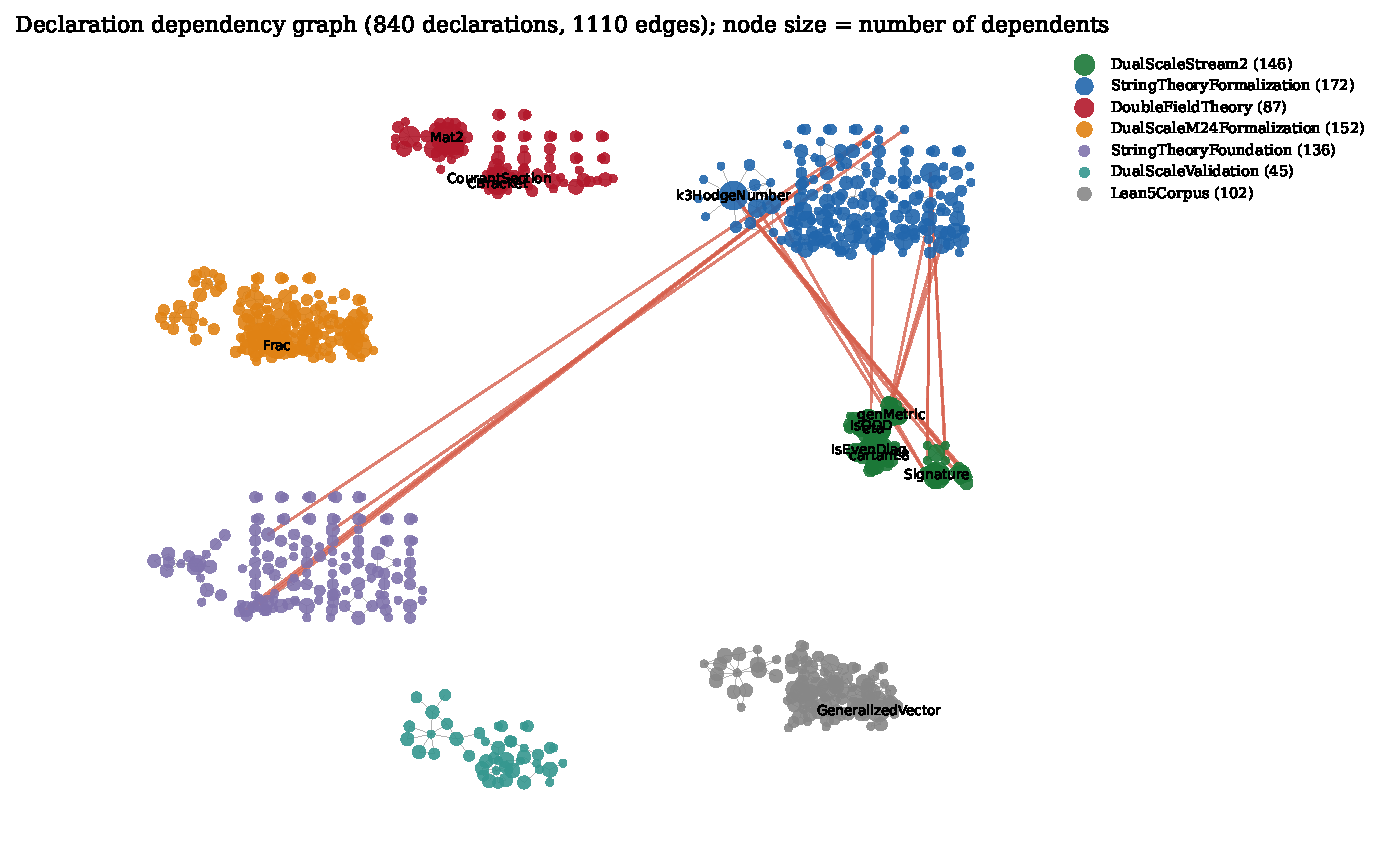
\includegraphics[width=\linewidth]{atlas_dependency_graph.pdf}
\caption{Kernel-level dependency graph of the declarations written in the source (isolated declarations omitted), one cluster per library (spring layout inside each cluster). Node size grows with the number of declarations that use it; the largest hubs are labelled. Red edges cross library boundaries: they are the bridges listed in the atlas chapter. \emph{Computed figure; data: \texttt{tools/lean\_depgraph.lean} (\texttt{.leancache/depgraph.jsonl}); layout: networkx Kamada-Kawai per connected component, one cluster per library.}}
\label{fig:atlas_dependency_graph}
\end{figure}
% [/fig:atlas_dependency_graph]
Full per-package tables are in \texttt{docs/STREAM2\_WORKFLOW.md} \S6; we summarize the pattern
here rather than re-deriving a single global percentage (the package-level goal counts there ---
26, 23, 10, and 6 goals for the lattice/T-duality pilot, the P2.3/P2.4-core/P2.5/P2.6 batch, the
P2.2 factorized-duality batch, and the dual-scale bound, respectively, summing to 65 of the
project's 99 theorems at the time of those runs --- are reported \emph{per package}, not as a global tier table; the
remaining goals were closed in later rounds, described qualitatively rather than re-tabulated, on
the mirror identity, section-condition, $SL(2,\mathbb{Z})$-product, $B$-shift, spectrum-equivalence,
reflection, and flux-integrality modules). The qualitative pattern was consistent and, in the
lattice pilot, sharp: the local prover closed essentially every \emph{concrete} goal (fixed
matrices, numerals, the 64-entry $E_8$ inverse check by \texttt{fin\_cases}, at a median latency of
4.4 s per attempt after a roughly 170 s one-time cold load) and \textbf{zero} of the eight
general-$n$/general-$d$ symbolic goals in that pilot. Haiku closed most short symbolic algebra with
an orchestrator-written proof sketch; Sonnet was needed only where a real mathematical idea was
required. The Sonnet share varied sharply by package rather than sitting at one corpus-wide rate:
in the lattice pilot, Sonnet closed 3 of 26 goals (11.5\%); in the P2.3/P2.4-core/P2.5/P2.6 batch,
8 of 23; in the P2.2 factorized-duality batch, 7 of 10; in the dual-scale bound, 2 of 6. A second
local model,
Goedel-Prover-V2-8B, closed zero goals in the pilot: with its thinking mode on it exhausted an
8192-token, 615-second budget without emitting an answer, and with thinking off it drifted off
target and emitted \texttt{sorry} scaffolds; this was recorded as a configuration failure at this
hardware's speed, not a capability verdict, and the model was dropped from routing.

\subsection{Honest failures}
The orchestrator throughout was a model (Opus) working under the author's direction, not a human
checking each step. We report below the false success reports that the gate \emph{caught}. We make
no claim about a detection rate: a misstatement the gate missed would, by construction, not appear in
this list, so ``all were caught'' is not something this method can establish. What the design does
guarantee is narrower and sufficient for Tier~A: no agent's report is ever counted, only a kernel
recompilation is, so a false report of success cannot by itself put an unproved statement into the
library. It gives no protection against a statement that compiles but says the wrong thing, which is
why statement review is a separate step. Three incidents are also too few to support a general
conclusion about language models and mathematics, and we draw none.

Two Haiku agent reports misstated their own compile status and were caught only because the
orchestrator recompiled every report before counting it (producer $\ne$ verifier, enforced, not
merely stated): one claimed five clean \texttt{sorry} placeholders while actually leaving eight
compile errors in \texttt{GeneralizedMetric}; another claimed ``no compilation errors'' in
\texttt{Factorized} while three proofs failed to parse. In the corpus's final round, a Haiku report
again claimed ``0 errors'' on the section-condition goals while one proof in fact failed to parse
due to an operator-precedence mistake, repaired by the orchestrator before the gate was re-run.
Separately, \texttt{lake env lean} (used by the single-file prover loop) does not apply
\texttt{lakefile.lean}'s \texttt{maxHeartbeats} option, so agents were, for a time, compiling under
a stricter timeout than the actual build uses; one Haiku agent abandoned the $E_8$ $LDL^{\mathsf T}$
goal on a heartbeat timeout that the real build budget does not hit, a lost-time bug rather than a
soundness one (a stricter gate can only reject valid proofs, never accept invalid ones). The route
chosen for a goal mattered as much as the tier assigned to it: \texttt{cartanE8\_posDef} failed
under Haiku via the literal 64-entry $L\cdot D\cdot L^{\mathsf T}$ matrix product, and was closed by
Sonnet only after the orchestrator reformulated it as the sympy-verified sum-of-squares identity
checked directly by \texttt{ring}. Finally, several block-matrix sign/transpose conventions ---
the $B$-shift covariance law, the mirror-symmetry matrix identity, the $O(d,d)$ pairing on
$J$ --- were checked with sympy before the corresponding Lean statement was written; this project
treats such a check as a useful pre-screen against a wasted proof attempt, and, per
\Cref{sec:tiers}, never as a substitute for the kernel proof itself.

%%%%%%%%%%%%%%%%%%%%%%%%%%%%%%%%%%%%%%%%%%%%%%%%%%%%%%%%%%%%%%%%%%%%%%%%%%%%%%%
\section{Conclusion}
\label{sec:conclusion}
%%%%%%%%%%%%%%%%%%%%%%%%%%%%%%%%%%%%%%%%%%%%%%%%%%%%%%%%%%%%%%%%%%%%%%%%%%%%%%%

\texttt{DualScaleStream2} kernel-certifies (Tier~A) the algebraic skeleton of $K3\times T^2$
T-duality and Double Field Theory: the positive-definiteness and unimodularity of the lattices
that build $H^2(K3,\mathbb{Z})$, the signature bookkeeping from $K3$ up through the Mukai and
$K3\times T^2$ charge lattices, the $O(d,d;\mathbb{Z})$ generators and their charge- and
spectrum-invariance for every torus dimension $d$, the Hull--Zwiebach generalized metric and its
$B$-shift and section-condition structure, a genuine real-analytic $d$-dimensional generalization
of this programme's dual-scale bound, flux-integrality and tadpole arithmetic on $K3\times T^2$
and $K3\times K3$, and the EOT elliptic-genus coefficient arithmetic against a Burnside-guarded
$M_{24}$ table. None of this proves that these objects constitute a string theory: the
identification of each formal object with its physical counterpart is drawn from the cited
literature or stated as this project's own conjecture, tier by tier, throughout. We consider the
value of this exercise to lie precisely in that separation --- and in the pipeline's own measured
failures (a symbolic goal the local prover cannot touch, an agent report that is simply false,
a build-configuration mismatch that silently over-constrains a proof search) being caught by a
kernel gate and a producer-independent verifier rather than by trust.

%%%%%%%%%%%%%%%%%%%%%%%%%%%%%%%%%%%%%%%%%%%%%%%%%%%%%%%%%%%%%%%%%%%%%%%%%%%%%%%
\appendix
\section{Reproducibility}
\label{app:repro}
%%%%%%%%%%%%%%%%%%%%%%%%%%%%%%%%%%%%%%%%%%%%%%%%%%%%%%%%%%%%%%%%%%%%%%%%%%%%%%%

\subsection{Build}
From the repository root:
\begin{center}
\footnotesize\ttfamily
lake build DualScaleStream2
\end{center}
completes in \textbf{3670 jobs} with no errors and zero \texttt{sorry} warnings, on toolchain
\texttt{leanprover/lean4:v4.33.1} with Mathlib \texttt{v4.33.1}. The library comprises
\textbf{19 modules} across the \texttt{Lattice}, \texttt{TDuality}, \texttt{DFT},
\texttt{DualScale}, \texttt{Flux}, and \texttt{Moonshine} namespaces (listed in
\Cref{sec:lattices,sec:tduality,sec:dft,sec:trace-bound,sec:flux,sec:moonshine}). Most of the
3670 jobs are Mathlib's own dependency graph, not this library's proof content; the job count is a
build-system measurement, not a count of theorems.

\subsection{Axiom audit}
\begin{center}
\footnotesize\ttfamily
python3 tools/axiom\_audit.py DualScaleStream2
\end{center}
reports \textbf{100 theorems}, \textbf{0 failing}, with every declaration's axiom footprint limited
to \texttt{propext}, \texttt{Classical.choice}, and \texttt{Quot.sound} --- Lean's three standard
axioms, no custom axiom, and no \texttt{sorryAx} or \texttt{native\_decide} anywhere in the
library. Stream~1 was re-gated in the same session for comparison: \texttt{lake build} 3353 jobs
across its six libraries, \textbf{326 theorems}, 0 failing (\texttt{DualScaleValidation} 23,
\texttt{Lean5Corpus} 53, \texttt{DoubleFieldTheory} 44, \texttt{StringTheoryFoundation} 56,
\texttt{DualScaleM24Formalization} 61, \texttt{StringTheoryFormalization} 89).

\subsection{Statement lock}
\begin{center}
\footnotesize\ttfamily
python3 tools/statement\_lock.py --check
\end{center}
verifies every theorem statement (up to its top-level \texttt{:=}) and every definition body
against a hash recorded in \texttt{docs/statement\_lock.json} at review time, so that replacing a
\texttt{sorry} with a proof cannot silently coincide with weakening the statement that was
reviewed.

\subsection{Roadmap coverage}
\texttt{docs/STREAM2\_WORKFLOW.md} \S5.1 records \textbf{18 of 18} planned roadmap items
(phases P2.1--P2.6) as done, each item meaning every theorem for it is committed, \texttt{sorry}-free,
and axiom-audited. As the workflow document itself stresses, this is 100\% \emph{of this plan},
counting items against a checklist this project wrote for itself --- not a fraction of ``string
theory,'' and not a claim of completeness for any of the physical theories discussed in
\Cref{sec:intro}.

\subsection{Scope of this appendix}
No number in this appendix was taken from memory: the job counts, theorem counts, and axiom
footprints above are the output of the commands shown, re-run at the commit recorded in this
paper's version history, and the phase/module correspondence matches
\texttt{docs/STREAM2\_WORKFLOW.md} \S5.1 and \S6 and \texttt{docs/PAPER\_REVISION\_BRIEF\_2026\_09\_17.md}
\S1, which a reader can re-run rather than trust.

\begin{thebibliography}{99}

\bibitem{Lean4Paper} L.~de Moura and S.~Ullrich, ``The Lean 4 Theorem Prover and Programming Language,'' in \textit{Automated Deduction -- CADE 28}, Springer (2021) 625--635.
\bibitem{Buscher1987} T.~H.~Buscher, ``Path-integral derivation of quantum duality in nonlinear sigma-models,'' \textit{Phys. Lett. B} 201 (1988) 466--472.
\bibitem{Buscher1988} T.~H.~Buscher, ``A symmetry of the string background field equations,'' \textit{Phys. Lett. B} 194 (1987) 59--62.
\bibitem{Narain1986} K.~S.~Narain, ``New Heterotic String Theories in Uncompactified Dimensions $<10$,'' \textit{Phys. Lett. B} 169 (1986) 41--46.
\bibitem{GiveonPorratiRabinovici1994} A.~Giveon, M.~Porrati, and E.~Rabinovici, ``Target space duality in string theory,'' \textit{Phys. Rept.} 244 (1994) 77--202, \textit{arXiv:hep-th/9401139}.
\bibitem{Aspinwall1996} P.~S.~Aspinwall, ``K3 Surfaces and String Duality,'' \textit{arXiv:hep-th/9611137} (1996).
\bibitem{HullZwiebach2009} C.~Hull and B.~Zwiebach, ``Double Field Theory,'' \textit{JHEP} 09 (2009) 099, \textit{arXiv:0904.4664}.
\bibitem{Huybrechts} D.~Huybrechts, \textit{Lectures on K3 Surfaces}, Cambridge University Press (2016).
\bibitem{DasguptaRajeshSethi1999} K.~Dasgupta, G.~Rajesh, and S.~Sethi, ``M Theory, Orientifolds and G-Flux,'' \textit{JHEP} 08 (1999) 023, \textit{arXiv:hep-th/9908088}.
\bibitem{GukovVafaWitten1999} S.~Gukov, C.~Vafa, and E.~Witten, ``CFT's From Calabi-Yau Four-folds,'' \textit{Nucl. Phys. B} 584 (2000) 69--108, \textit{arXiv:hep-th/9906070}.
\bibitem{EguchiOoguriTachikawa2011} T.~Eguchi, H.~Ooguri, and Y.~Tachikawa, ``Notes on the K3 Surface and the Mathieu Group $M_{24}$,'' \textit{Exper. Math.} 20 (2011) 91--96, \textit{arXiv:1004.0956}.
\bibitem{Gannon2016} T.~Gannon, ``Much ado about Mathieu,'' \textit{Adv. Math.} 301 (2016) 322--358, \textit{arXiv:1211.5531}.
\bibitem{Callens2026Paper7} X.~Callens and the SocrateAI Agora Collaboration, ``The Dual-Scale String Theory: Mechanized Foundations, Singularity Resolution, Mathieu Moonshine, and a Zero-Free-Parameter Cosmological Conjecture on $K3\times T^2$,'' \textit{SocrateAI Laboratory for Mathematical Physics \& Formal Verification} (2026), \url{https://github.com/xaviercallens/SocrateAI-Scientific-Agora-LeanMaster}.

\end{thebibliography}

\end{document}
